\documentclass[conference]{IEEEtran}
% If the IEEEtran.cls has not been installed into the LaTeX system files,
% manually specify the path to it.  e.g.
% \documentclass[conference]{./IEEEtran}

% Add and required packages here
\usepackage{graphicx,times,amsmath}
\usepackage{verbatim} % for comments 
\usepackage{url} % for urls
\usepackage{rotating}% for text rotation
\usepackage{multirow} % 

\graphicspath{{images/}}   % where are the EPS images?


% Correct bad hyphenation here
\hyphenation{op-tical net-works semi-conduc-tor IEEEtran}

% To create the author's affiliation portion using \thanks
\IEEEoverridecommandlockouts

\textwidth 178mm
\textheight 239mm
\oddsidemargin -7mm
\evensidemargin -7mm
\topmargin -6mm
\columnsep 5mm

\begin{document}

% Project title: keep the \ \\ \LARGE\bf in it to leave enough margin.
\title{\ \\ \LARGE\bf Starcraft: Evolving the Combat System}

\author{David Schedl \\ dacs@itu.dk \and Prakash Prasad \\ prpr@itu.dk \and Kacper Kokoszka \\ kjak@itu.dk }

% Uncomment out the following line for invited papers
%\specialpapernotice{(Invited Paper)}

% Make the title area
\maketitle
%-----------------------------
%  ABSTRACT
%-----------------------------
%\begin{abstract}
%\end{abstract}



%-------------------------------------------------------------------------------------------------------------------------------------------------
\section{Introduction}
\label{sec:Intro}
%-------------------------------------------------------------------------------------------------------------------------------------------------
%\PARstart{I}{f}
This report is an analysis of the various levels of combat involved in Starcraft: Brood War (SC)%
\footnote{\url{http://us.blizzard.com/en-us/games/sc/}} %
and how machine learning methodologies can be utilized to increase their efficiency.
%-------------------------------------------------------------------------------------------------------------------------------------------------
\subsection{Starcraft - The Game}
SC is a Real-Time Strategy (RTS) game that has huge fan-fare because of highly diverse, yet balanced game mechanics. The game features three different races - \emph{Terran}, \emph{Protoss} and \emph{Zerg}, each with special abilities, strengths and weaknesses. The gameplay revolves around mechanics to collect resources, build buildings, and build fighting units. The goal of a play session is to destroy all buildings of the opponent with your offensive forces. The offensive units however are so finely tuned that a player can easily win a battle, if he has the correct unit composition to his opponent. There are multiple permutations of such strategies, a handful of the most popular and efficient of these are collected in on-line compendium by fans and pro-gamers (like Team Liquid Forums%
\footnote{\url{http://wiki.teamliquid.net/starcraft/Strategy}}%
).

%-------------------------------------------------------------------------------------------------------------------------------------------------
\subsection{Artificial Intelligence}
%Competitions
The level of meta-game that evolves from SC is also intriguing from the aspect of AI. In-fact, there are several competitions held for AI bots playing SC, such as \emph{CIG 2010 Starcraft RTS AI Competition}%
\footnote{\url{http://ls11-www.cs.uni-dortmund.de/rts-competition/starcraft-cig2010}}%
, which was part of the Computational Intelligence in Games Conference, 2010. Another one is the \emph{Starcraft AI competition}%
\footnote{\url{http://eis.ucsc.edu/StarCraftAICompetition}}%
, which was part of the program at the 2010 conference on Artificial Intelligence and Interactive Digital Entertainment (AIIDE 2010). The complex and concurrent levels of controls operating in the game require a plethora of AI techniques to work together at all times. In application, RTS bots have a reputation for being extremely predictable and hence, human players find them very easy to beat. The CIG Starcraft AI competition challenges such bots to fight each other in a "Tech-Limited" game. The ruleset stipulates that it is a \emph{Terran} Vs \emph{Terran} game with only a subset of units and buildings allowed to be built. In order for an AI bot to play the full game effectively, it needs to take several kinds of sub-actions that can make him superior to the opponent.

%-------------------------------------------------------------------------------------------------------------------------------------------------
\subsection{Levels of Control}
%Levels of Controls
Lets try to break down important actions that an AI bot would have to take into levels of control:
\begin{description}
  	\item[Micro (Micro-Management):] \hfill \\ 
In SC terminology, \emph{Micro} refers to the capability of the human player to manage his units. These can be further classified into two types of micro objectives - offensive or non-offensive. Non-offensive micro is concerned with managing the units gathering minerals and on some occasions, using these units to block the opponent's offensive units to get an advantage. In SC, all offensive units are designed to do a higher than normal damage to particular units of the opponent. Skill in the game is attributed to finding out the unit composition that the opponent is going for, and then build the specific unit that can counter it. However, once these units have been build, they need to be ordered correctly to do the maximum damage.
  	\item[Squad Management:] \hfill \\
This is another dimension of the micro-management, which takes control of giving commands to a group of units in battle with an opposition squad. Managing the arrangement and attack/withdraw schema of the units in the squad can mean the difference between victory and losing. Moreover, efficient control also minimizes the loss of resources used in building these units.
  	\item[Scouting:] \hfill \\
As in any game, an important part of efficiently playing the game is knowledge about its state. In terms of SC, this involves knowing what the opponent is upto. The game implements a \emph{Fog of War} over areas that the player does not have units in. This means the player has to carry out scouting on the map over time to keep himself aware of the opponent's actions.
	\item[Overall Strategy:] \hfill \\
Once a player has information about the opponent's mineral harvesting capabilities, bases, building structures and units being generated, decisions need to be made such as which units to generate (which in turn needs to evaluate corresponding buildings needed to be built), expansion of bases (for higher mineral harvesting rate), attack timing, and path-finding (and blocking choke points for defense). These decisions keep the overall coherence of the bot's strategy. In SC lingo, this potion of the game is often classified as \emph{Macro}.
\end{description}

In this report we will focus on combat mechanics of Starcraft, where we analyze the game's levels of controls in terms of fighting, applicable only within the scope as defined under the CIG Starcraft AI Competition ruleset.


%-------------------------------------------------------------------------------------------------------------------------------------------------
\subsection{Units}
%
%	STUFF ABOUT UNITS
%

%
% ---------
\begin{table*}[htb]
\caption{Unit statistics}
\begin{center}
% Table generated by Excel2LaTeX from sheet 'Sheet1'
\begin{tabular}{|l|r|r|r|r|r|r|r|r|r|}
\hline
           &            &            &            &            &            &            &        \multicolumn{3}{|c|}{\bf Attack} \\
\multicolumn{1}{|c|}{\bf Unit} &  
\multicolumn{1}{|c|} {\bf HP} & 
\multicolumn{1}{|c|}{\bf Armor} & 
\multicolumn{1}{|c|}{\bf Size} & 
\multicolumn{1}{|c|}{\bf Speed} & 
\multicolumn{1}{|c|}{\bf Range} & 
\multicolumn{1}{|c|}{\bf Cooldown} & 
\multicolumn{1}{|c|}{\bf Damage} & 
\multicolumn{1}{|c|}{\bf Times} & 
\multicolumn{1}{|c|}{\bf Type} \\
\hline
{\it Marine} &         40 &          0 &      Small &          4.00 &          4 &         15 &          6 &          1 &     Normal \\
\hline
{\it Firebat} &         50 &          1 &      Small &          4.00 &          2 &         22 &          8 &          2 & Concussive \\
\hline
{\it Goliath} &        125 &          1 &      Large &       4.57&          6 &         22 &         12 &          1 &     Normal \\
\hline
\end{tabular}  
\label{table:units}
\end{center}
\end{table*}
% ---------
%
SC has different types of units each having different abilities. Table \ref{table:units} gives an overview of units we use in our tests. One of the important facts, which can be found in this table, is the damage a unit gives to another unit when it is attacking. Due to the balancing of the game, there are three different weapon types which cause a different amount of damage to units, depending on the size of the opponent unit. Table \ref{table:multiplier} shows these multipliers. To finally calculate the discount of hit points a unit receives the following equation:
%	Potential Damage = (Damage - Armor) * Multiplier										
\begin{align}
	hp discount &= (damage \cdot times - armor) \cdot multiplier
	\label{equation:damage}
\end{align}
must be applied, where the $damage$ is the {\bf Damage} value of the attacking unit in Table \ref{table:units}, $times$ is the {\bf Attack Times}  of it, $armor$ is the {\bf Armor} of the defending unit and $multiplier$ is the value from Table \ref{table:multiplier}. 
To make this clearer we calculate a small example, where a {\it Firebat} shoots at a {\it Goliath}. A {\it Firebat} can shoot two times with a damage of $8$ which results in a damage sum of $16$. From that we have to subtract $1$ because the {\it Goliath} has an armor of $1$. The multiplier from Table \ref{table:multiplier} is $0.25$ because the {\it Firebat} has concussive damage and the {\it Goliath} has a large unit size. Therefore the final damage that the Firebat causes a Goliath is $3.75$, per attack.
%(16-1)*0,25
%

% ---------
\begin{table}
\caption{Multiplier depending on weapon types and on the unit size}
\begin{center}
% Table generated by Excel2LaTeX from sheet 'Sheet1'
\begin{tabular}{|l|r|r|r|}
\hline
\multicolumn{1}{|c|}{\bf Unit Size } & 
\multicolumn{1}{|c|}{\bf Concussive } &    
\multicolumn{1}{|c|}{\bf Normal } & 
\multicolumn{1}{|c|}{\bf Explosive } \\
\hline
{\it Small} &          1.00 &          1.00 &        0.50 \\
\hline
{\it Medium} &        0.50 &          1.00 &       0.75 \\
\hline
{\it Large} &       0,25 &          1.00 &          1.00 \\
\hline
\end{tabular}  
\label{table:multiplier}
\end{center}
\end{table}
% ---------


%
%	STUFF ABOUT Broodwar API
%
Implementation of the bot in this project is done using BWAPI\footnote{\url{http://code.google.com/p/bwapi/}} %
which is a free framework used to enable communication with SC (patch $1.16.1$). BWAPI provides functionalities to interact with the game like a human player, therefore it is suitable for developing AI bots. The API uses DLL injection to simulate the actions of a human player while reading all aspects of the game state. As with the language of the framework, all code for the project is written in C++. Additionally, BWSAL (Standard Add-on)\footnote{\url{http://http://code.google.com/p/bwsal/}} %
and BWTA (Terrain Analyzer)\footnote{\url{http://code.google.com/p/bwta/}} %
are used to enhance the information known about the game.
% MORE? LESS?

%/************************************************************************************************
\begin{comment}
%
% THIS IS HOW YOU DEFINE A FIGURE - SAMPLE
%%
\begin{figure}[htp]
\centerline{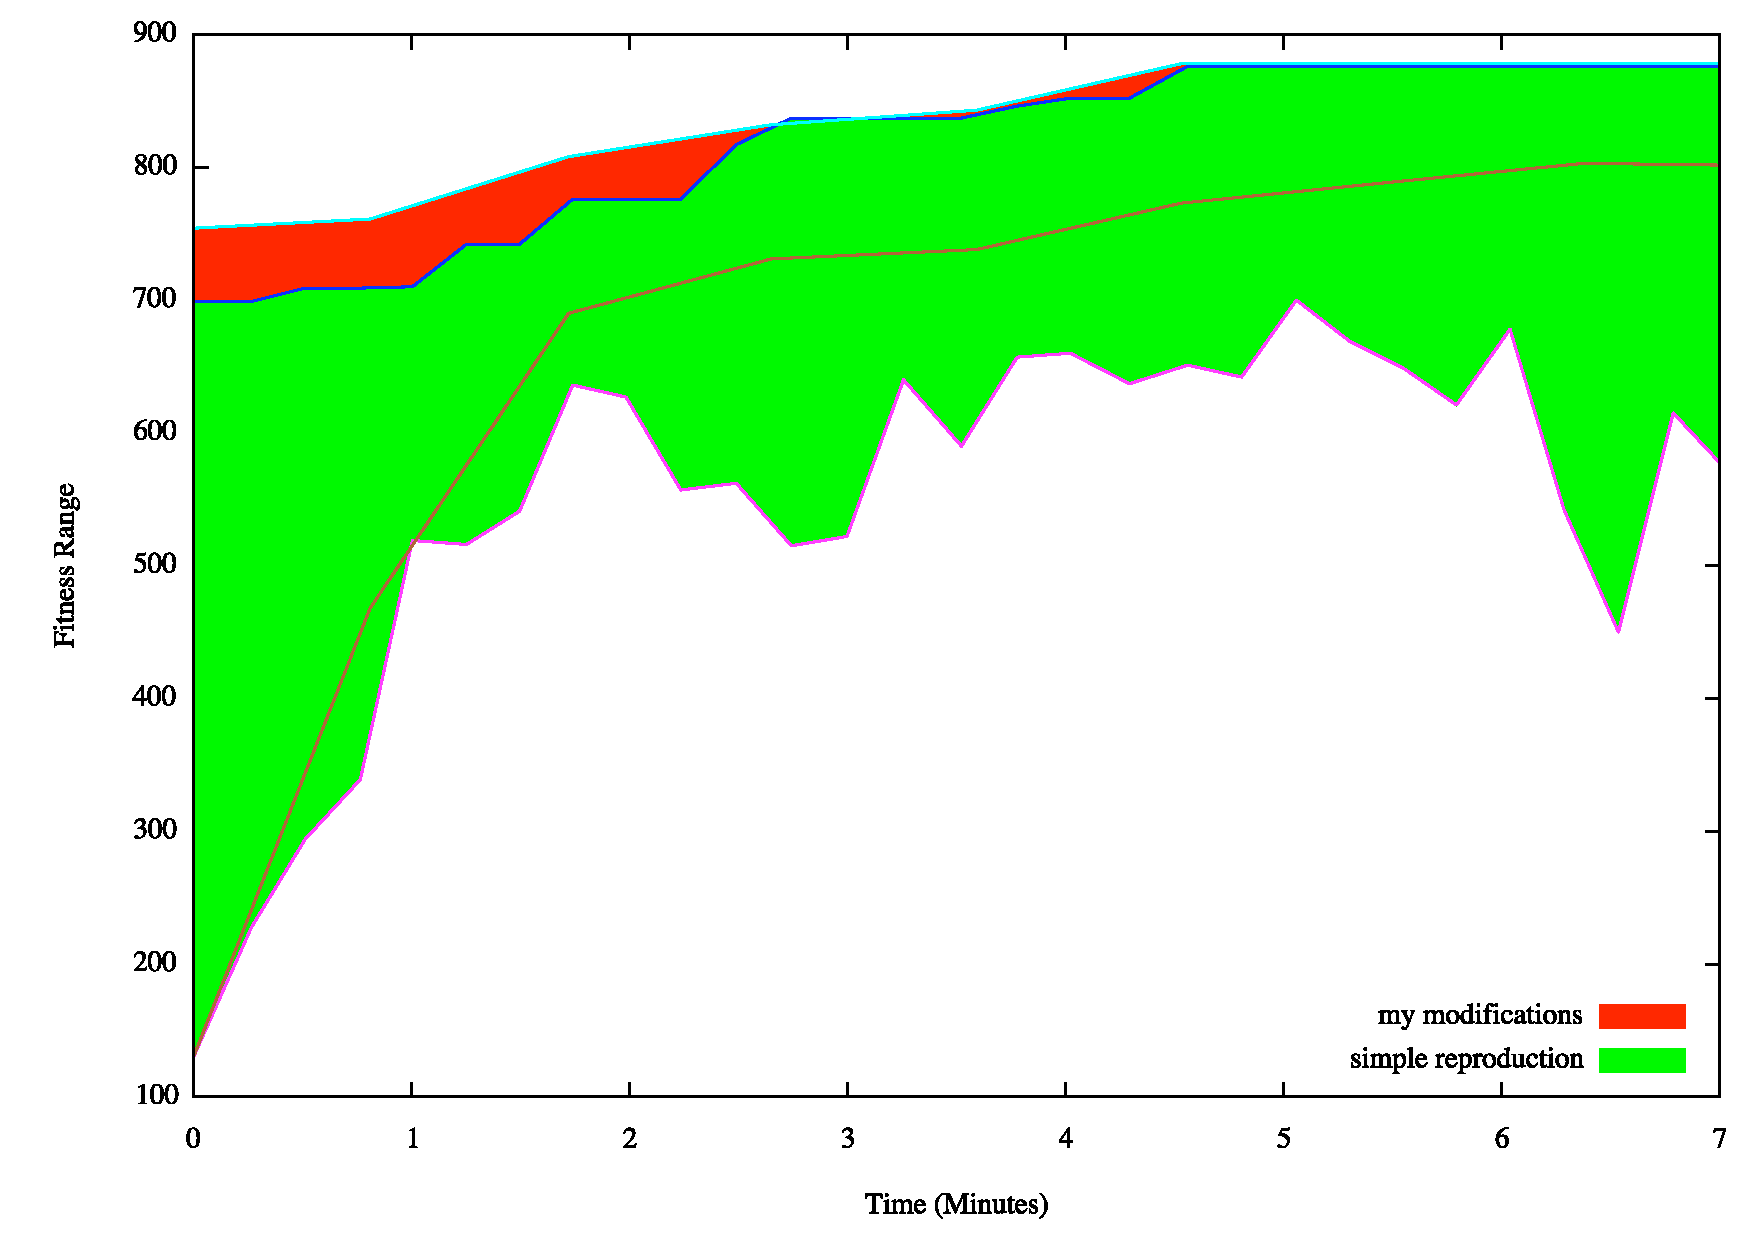
\includegraphics[width=1.0\columnwidth]{fig_gaComparison}}
\caption{Caption of a figure}
\label{fig:comparison}
\end{figure}
%%

\end{comment}
%************************************************************************************************/

% CAN THIS SECTION BE ANY GOOD? OR IS IT USELESS?
% A common Random player is presented to show the fighting mechanism
% Main-Author: Prakash
%
%-------------------------------------------------------------------------------------------------------------------------------------------------
\section{Random Player}
%-------------------------------------------------------------------------------------------------------------------------------------------------

%-------------------------------------------------------------------------------------------------------------------------------------------------
\subsection{One Unit Vs One Unit Combat} 
To fulfill the offensive objectives for the game players fight their units against the opponent's. The procedural execution of a fighting loop is as follows:
\begin{description}
	\item[Unit Actions:] \hfill \\ 
At any given point, a unit in SC can take any one of the following orders:
\begin{itemize}
\item Move
\item Attack
\item Hold Position
\item Unit Specific Orders - These are special orders which are different for all units. For the sake of this project, we disregard these commands.
\end{itemize}
  	\item[Unit Attack Range:] \hfill \\ 
A unit can only attack units within its weapon range.
  	\item[Damage, Armor and Damage Multiplier:] \hfill \\
Once in range, and only if the unit decides to attack, the damage multiplier logic explained in Table \ref{table:multiplier} is used to calculate the damage taken by the unit attacked and processed immediately.
  	\item[Cooldown:] \hfill \\
After each attack action, the unit needs to spend certain number of update cycles before it can attack again.
	\item[Speed:] \hfill \\
In case the unit decides to move, the unit can move at a specific speed.
\end{description}
In order to see the complexity and non-trivial nature of the task of commanding a unit in battle, a test case was established. In this scenario, an AI bot unit fights the SC game AI unit. The bot makes a random command decision on each frame out of the possible actions of either retreating away from the enemy or attacking the enemy.
%%%

%-------------------------------------------------------------------------------------------------------------------------------------------------
\subsection{Results} 
During the tests conducted with the model explained above, the random bot only won $1$ game out of $1000$ tests carried out. Unlike a stochastic game such as LUDO, where random chance controls the outcome of a game, SC is highly deterministic where a random bot cannot depend on chance to win a match. This goes to prove that a random bot is not effective at fighting in SC, and raises the need for better computational intelligence strategies for processing unit commands.
%%%

%
% INPUT
% everything related to Reinforcement Learning
% Main-Author: Kacper
%
%-------------------------------------------------------------------------------------------------------------------------------------------------
\section{Reinforcement Learning}
\label{section:RL}
%-------------------------------------------------------------------------------------------------------------------------------------------------

%-------------------------------------------------------------------------------------------------------------------------------------------------
\subsection{Method} \hphantom{x}
In our first approach we focused on Micro-management in one versus one battles using combination of artificial neural network and reinforcement learning. The general idea was to create neural network that decides which action is going to be executed while reinforcement learning would be responsible for teaching neural network a proper strategy - the desired output values for neural network backpropagation are delivered reward mechanism of reinforcement learning. More information about reinforcement learning can be found in \cite{aSurvey}. \\ \hphantom{x}
In our final solution we decided that there are two basic decisions to be made: attack which order our bot unit to engage enemy unit or withdraw which order our bot unit to move in direction opposite to enemy position. Therefore there were two neural networks created. Each network is responsible for each decision. and the action with neural network higher output value is selected.
\\
\subsubsection{Representation}\hfill \\ \hphantom{x}
During the implementation and first tests processes a number of different inputs were considered as a state representation. All the considered inputs are going to be presented in order of better understanding of input experiments. \\ \hphantom{x}
The following inputs are the general inputs:
\begin{description}
\item[Distance state] \hfill \\
This idea was to represent a distance between two fighting units with four discrete states:
\begin{itemize}
	\item when our unit is in enemy weapon range and enemy unit is not in our weapon range,
	\item when both units are out of their weapon range,
	\item when both units are in their weapon range,
	\item when enemy unit is in our weapon range and our unit is not in enemy weapon range,
\end{itemize}
\item[Continuous distance]\hfill \\
The distance between units is an continuous distance provided by game engine and normalized with number 500.0 and later by number 250.0,
\begin{IEEEeqnarray}{rCl}
cd=\frac{dbu}{250.0},
\end{IEEEeqnarray}
where: \\
cd - continuous distance, \\
dbu - distance between units,
\item[Previous action] \hfill \\
Provides an information about previous action taken.
\end{description}
\hfill \hphantom{x} The following inputs are personalized for each unit - one is the set of information about our bot unit and the second is a set of information about enemy unit:
\begin{description}
\item[Health (hit points)] \hfill \\
Provides an information about current unit health, the value is normalized with max unit HP value,
\begin{IEEEeqnarray}{rCl}
hp=\frac{cuhp}{muhp},
\end{IEEEeqnarray}
where: \\
hp - health,\\
cuhp - current unit health,\\
muhp - maximum unit health,
\item[Damage] \hfill \\
Informs about damage amount that unit is able to cause to enemy unit, the value is normalized by maximum value of both unit damage amount,
\begin{IEEEeqnarray}{rCl}
d=\frac{ud}{\max\{ud, od\}},
\end{IEEEeqnarray}
where:\\
d - damage,\\
ud - unit damage,\\
od - opponent unit damage,
\item[Weapon range] \hfill \\
Is an information about unit weapon range, the value is normalized by maximum value of both unit weapon range,
\begin{IEEEeqnarray}{rCl}
wr = \frac{uwr}{\max\{uwr, owr\}},
\end{IEEEeqnarray}
where:\\
wr - weapon range,\\
uwr - unit weapon range,\\
owr - opponent unit weapon range,
\item[Current cooldown] \hfill \\
Provides an information about a time that is left until unit would be able to attack again, the value is normalized by maximum unit cooldown value,
\begin{IEEEeqnarray}{rCl}
cc = \frac{ucc}{muc},
\end{IEEEeqnarray}
where:\\
cc - current cooldown,\\
ucc - unit current cooldown,\\
muc - maximum unit cooldown,
\item[Max cooldown] \hfill \\
Provides an information about maximum time left until unit would be able to attack again, the value is normalized by maximum value of both unit maximum cooldown,
\begin{IEEEeqnarray}{rCl}
mc = \frac{muc}{\max\{muc,moc\}},
\end{IEEEeqnarray}
where:\\
mc - maximum cooldown,\\
muc - maximum unit cooldown,\\
moc - maximum opponent unit cooldown,
\item[Top speed] \hfill \\
The maximum unit speed value, the value is normalized by maximum value of  both unit top speed values,
\begin{IEEEeqnarray}{rCl}
ts = \frac{uts}{\max\{uts, ots\}},
\end{IEEEeqnarray}
where:\\
ts - top speed,\\
uts - unit top speed,\\
ots - opponent unit top speed,
\item[Distance to enemy] \hfill \\
Provides information about distance to opponent unit, normalized in following manner:
\begin{itemize}
\item if the enemy unit is in weapon range than values from -1 up to 0 are provides where -1 is very close to opponent unit and 0 is on the edge of unit weapon range,
\item if the opponent unit is out of the unit weapon range than values form 0 up to 1 are provided where 0 is on the edge of unit weapon range and 1 is unit weapon range multiplied by two.
\end{itemize}
\begin{IEEEeqnarray}{rCl}
dte = \min\{1.0, \frac{dbu-ur}{2 \times ur}\},
\end{IEEEeqnarray}
where:\\
dte - distance to enemy,\\
dbu - distance between units,\\
ur - unit range.
\end{description}
\hfill \\

\subsubsection{QLearning}\hfill \\ \hphantom{x}
Rewarding mechanism was divided into two parts. \\ \hphantom{x}
The first part was big reward for winning (of value 1) and big penalty for loosing at the end of match (of value -1). \\ \hphantom{x}
The second part are the rewards and penalties provided during the match. Again, we tested multiple approaches in this area:
\begin{description}
\item[Hit opponent, loose hp] \hfill \\
In this case the idea was to reward bot for hitting enemy with  reward of small value and punish bot for loosing hit points also with a small value,
\item[Units hp comparison] \hfill \\
This approach base on comparison of our and enemy unit hit points. If our unit have more or equal hit points compared to enemy unit than bot was rewarded with a small value reward. In other case (less hit points than enemy), bot was punished with a small value punishment.
\item[Modified hp comparison] \hfill \\
The modification of the previous approach was made in two aspects. First of all, the rewards and penalties are now continuous instead of discrete as in both previous cases and second - values of rewards are close to big penalty and big reward. The formula that provides this values is presented by equation below (\ref{equation:reward_a}):
\begin{IEEEeqnarray}{rCl}
r = \frac{uhp-ehp}{\max\{uhp, ehp\}},
\label{equation:reward_a}
\end{IEEEeqnarray} 
where:\\
r - reward,\\
uhp - unit hit points,\\
ehp - enemy unit hit points.\\
The equation output are values from -1 to 1, where -1 means big punishment, 0 means no reward at all and 1 means big reward.
\end{description}
\hfill \\ \hphantom{x}
There are two parameters for our implementation of QLerning. The discount factor parameter which determines the importance of future rewards was set at the end to 0.9. The $\varepsilon$ parameter necessary for $\varepsilon$-greedy mechanism, which was also implemented, was at the end set to 0.01. \\

\subsubsection{Neural Network}\hfill \\ \hphantom{x}
As it was mentioned at the beginning of this section, in order to handle two possible actions, we decided to create two separate neural networks, each responsible for one action.
\\ \hphantom{x}
The structure of neural network was kept simple. The number of neurons in middle layer was half of inputs into network and the output was only one. The learning rate was set to 0.05.

%%%

%-------------------------------------------------------------------------------------------------------------------------------------------------
\subsection{Results}  \hfill \\ \hphantom{x}
All test were provided for matches played between two marine units.\\

\subsubsection{Inputs and reward mechanism experiments}\hfill \\ \hphantom{x}
First results of preliminary tests revealed that our first ideas about state representation and reward mechanism were missed. Therefore we decided to provide additional tests in those areas. Testing methodology was iteration of 40 matches where 30 first of them were the exploration part and last 10 were exploitation part. Based on data received this way we were able to create line graphs of won matches over all iterations played. \hfill \\ \hphantom{x}
First version of state representation included all mentioned inputs, except of \emph{Distance state} and \emph{Distance to enemy}. For the rewarding mechanism during the match \emph{Hit opponent, loose hp} approach was chosen. Unfortunately, first results represented on Fig.\ref{fig:first} revealed that this representation was not good configuration. The information received by bot player were not properly adjusted to enable him to learn particular strategy.
\\ \hphantom{x}
Next test were made with almost the same as previously representation - \emph{Continuous distance} was replaced by \emph{Distance state}. The rewarding mechanism remained the same. This time the results, which are presented on Fig.\ref{fig:first}, appeared to be bad and even worse that in previous test. The bot had a problem with recognizing best area to stay in - most of the time he was fluctuating between both units in weapon range area and both unit out of weapon range area. Based on this test and couple of more further tests we decided to ultimately abandon \emph{Distance state} input.
\begin{figure}[htp]
\centerline{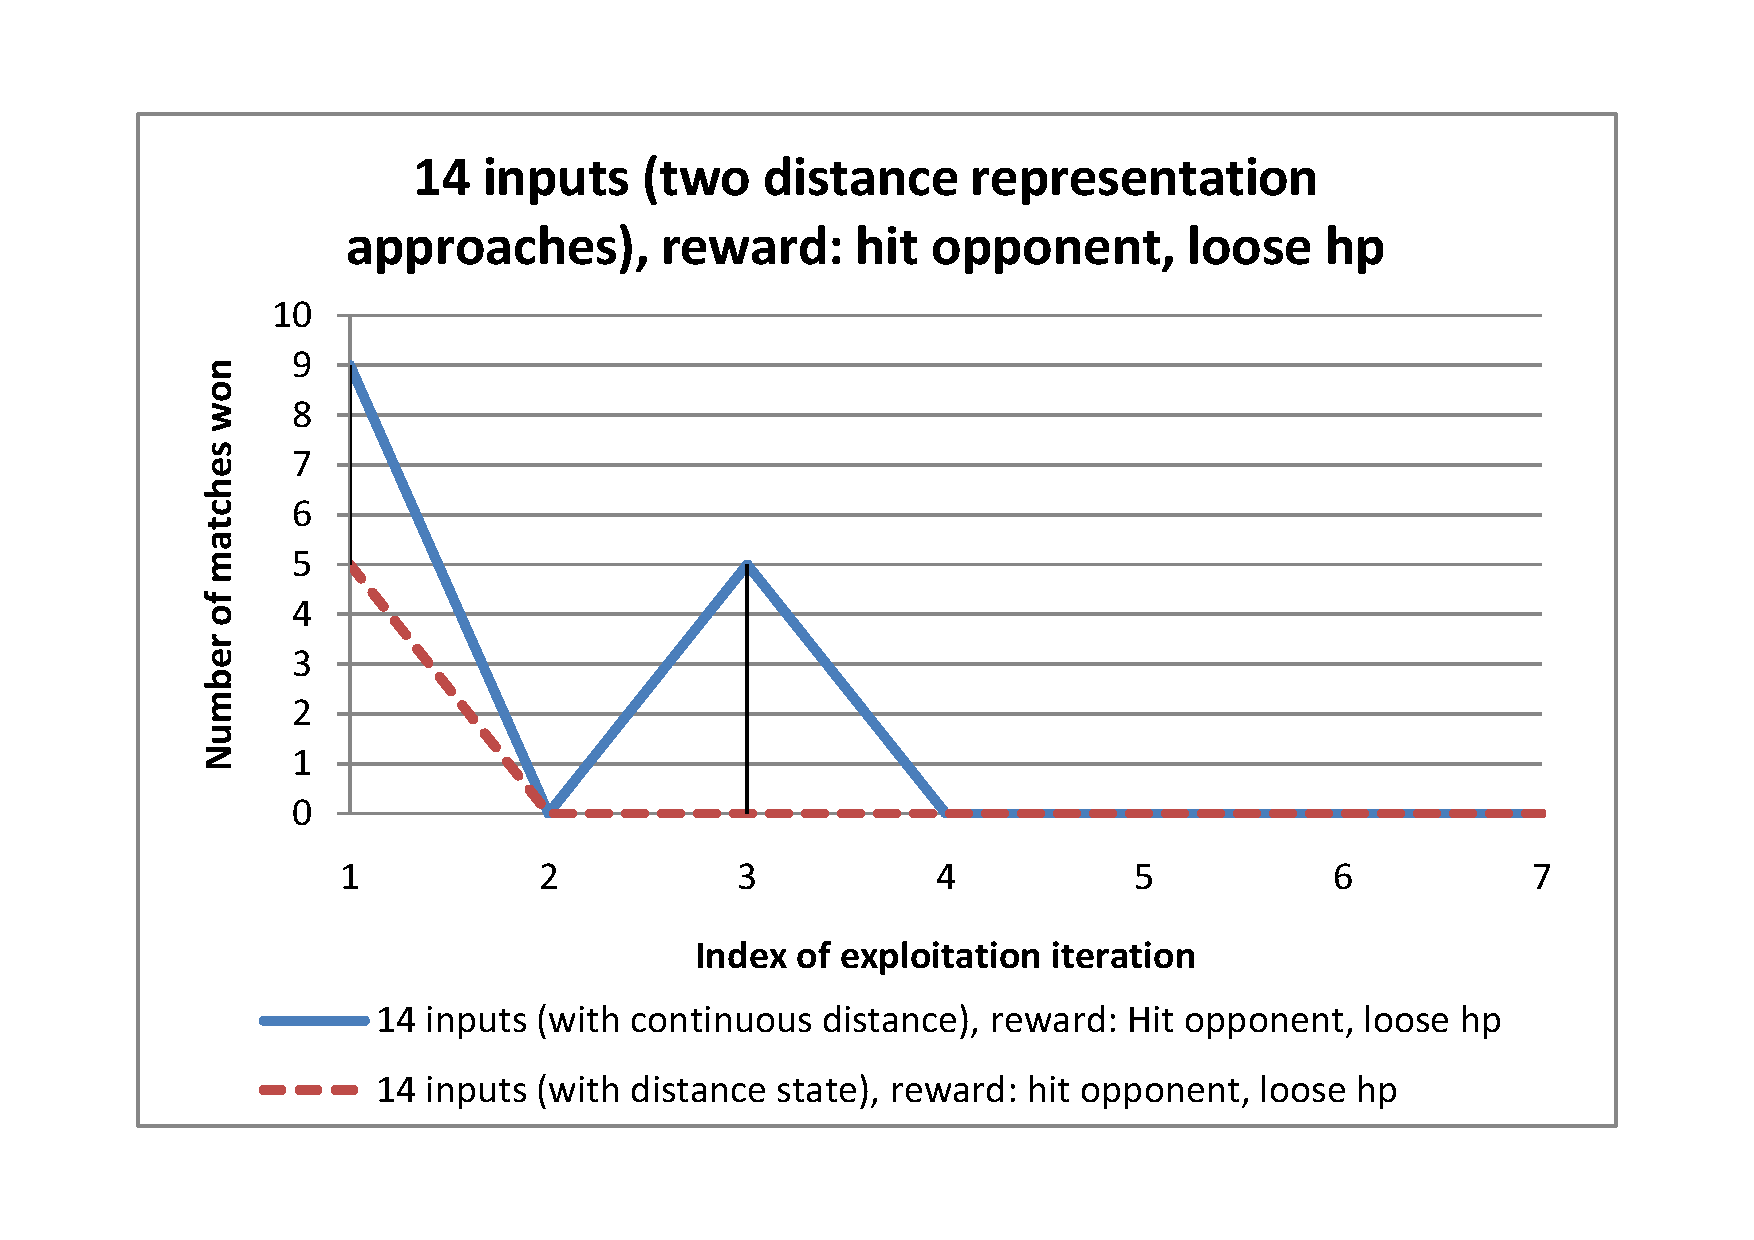
\includegraphics[width=1.0\columnwidth]{fig_ql_14_r1}}
\caption{Results of tests: 14 inputs (two distance representation approaches), reward: Hit opponent, loose hp}
\label{fig:first}
\end{figure}
%%
\\ \hphantom{x}
We decided to turn in the rewarding mechanism changes direction. Once more two previously tested representations were used but with \emph{Unit hp comparison} approach. Also a small change were made to representation - we decided to drop top speed input as well in order to smaller representation. This time one of the results appeared to be promising and is presented on Fig.\ref{fig:third}.
\begin{figure}[htp]
\centerline{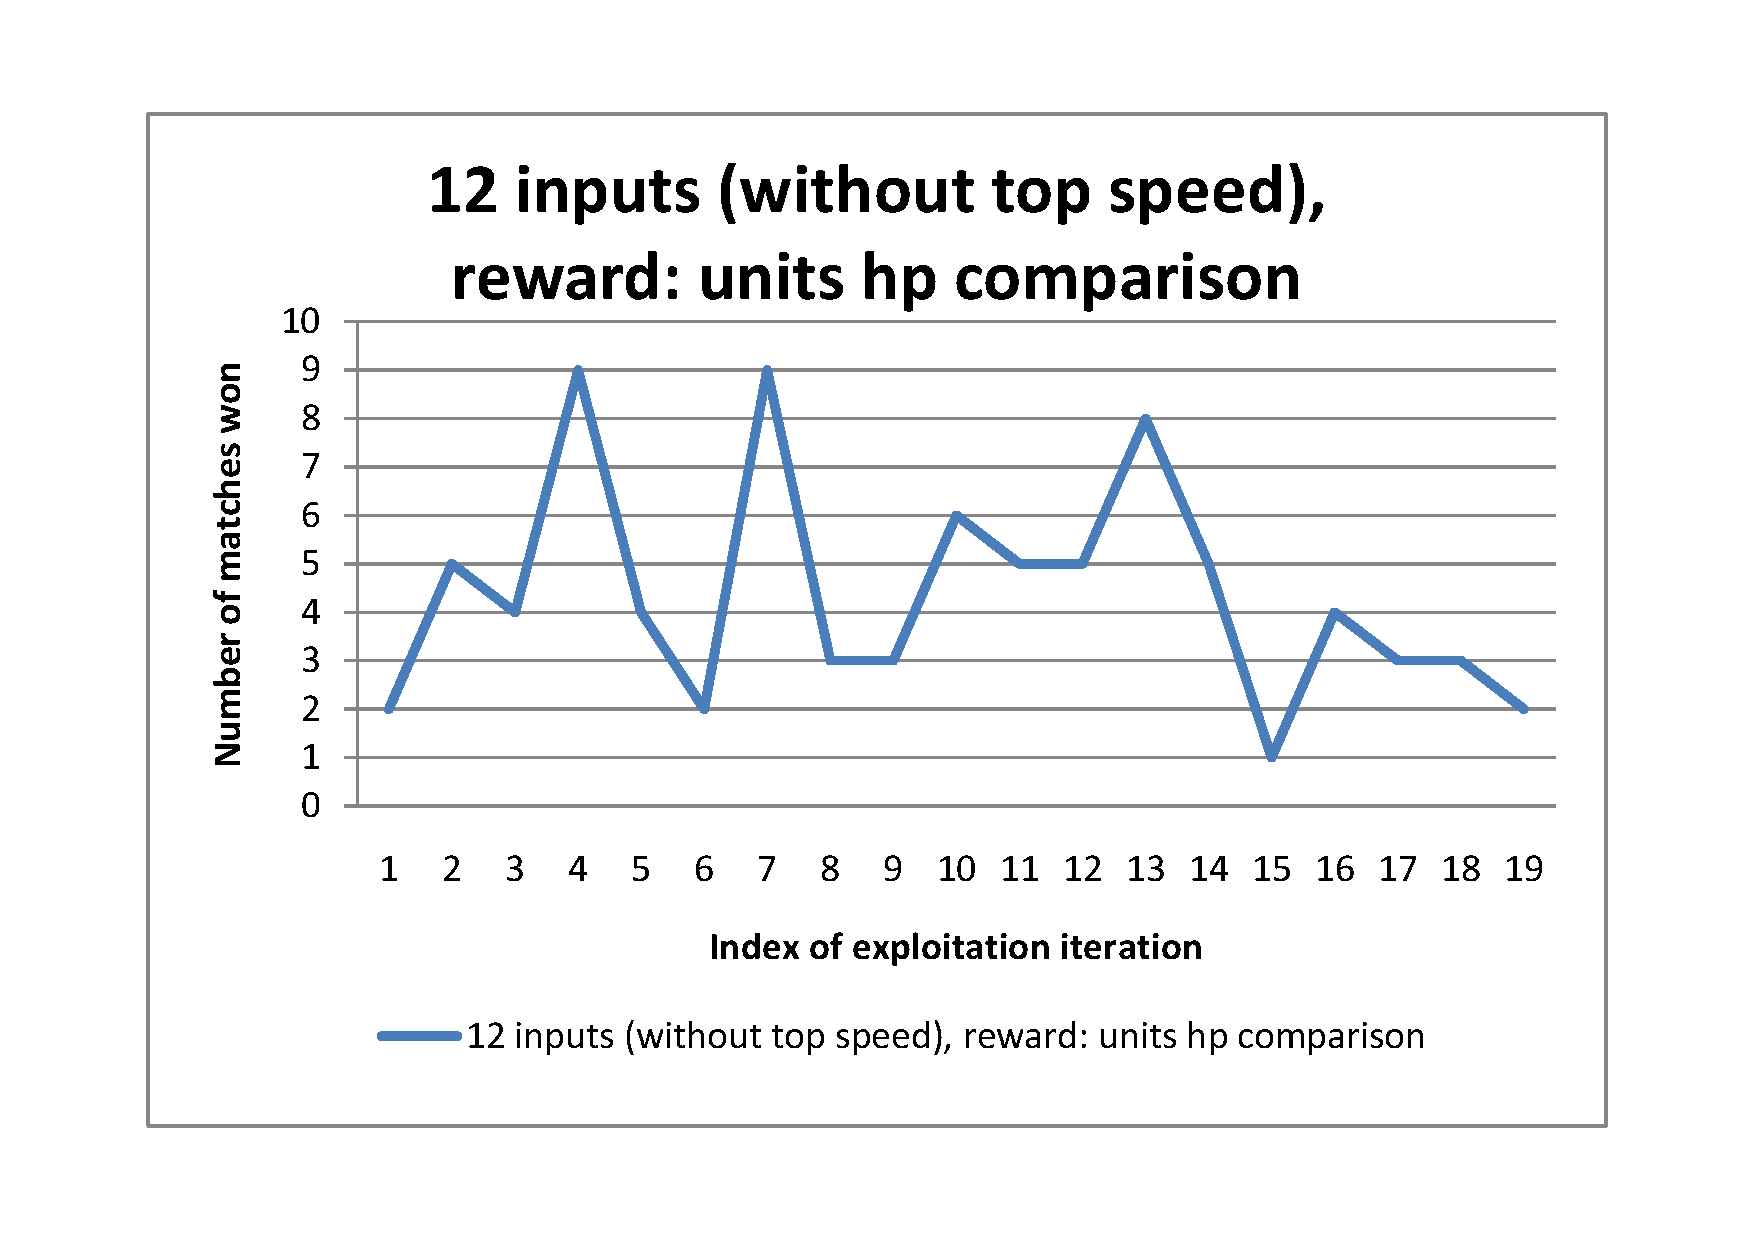
\includegraphics[width=1.0\columnwidth]{fig_ql_12(-ts)_r2}}
\caption{Results of test: 12 inputs (without top speed), reward: Hit opponent, loose hp}
\label{fig:third}
\end{figure}
%%
\\ \hphantom{x}
At this figure we can see that in first few iterations bot starts to learn some strategy - winning rate is rising, but later winning rate starts floating from 2 won matches up to 9 won matches. At the end winning rate starts to strive for zero. Once more selected state representation and reward mechanism appears to be not a good combination.
\\ \hphantom{x}
In order to receive more information, more excluding certain inputs and switching rewarding mechanism tests were provided. Unfortunately, the results were not satisfying, however enabled us to understand bot working mechanisms better.
\\ \hphantom{x}
At the end we decided to rearrange reward mechanism entirely and also smaller representation state. The final version included only 7 inputs: \emph{Previous action},\emph{ Health}, \emph{Current cooldown} and\emph{ Distance to enemy}. The rewarding mechanism, instead of approaches with small reward value, were changed into \emph{Modified comparison} mechanism. Both this changes allowed to achieve promising and effective results presented on Fig.\ref{fig:nnfr} and Fig.\ref{fig:nnff}. From those figures we are able to perceive learning process. More comment on results of this test is to be found in next section (NN structure experiments) under 7-3-1 neural network structure test.
\\
\subsubsection{QL parameters experiments}\hfill \\ \hphantom{x}
Q learning in our implementation requires two parameters: discount factor which is a multiplier factor for maximum future value and $\varepsilon$ which is a $\varepsilon$-greedy mechanism parameter. \\ \hphantom{x}
Tests with first mentioned parameter revealed that with it's increasing value teaching abilities of reinforcement learning increases. With the discount factor of value 0.5 neural network was not able to learn proper wining strategy - the only strategy the bot came up with was attacking for a short time and withdrawing a little. Theoretically this strategy might be a good one, but during the real match bot was not able to perform all this actions in a way so this strategy would be effective - bot was dying most of matches. We achieved best results with a discount factor of value 0.9. \\ \hphantom{x}
Testing $\varepsilon$ parameter revealed that with it's bigger value bot's performance weakens. According to random bot, described in previous chapters where we shown that random player approach is entirely inefficient, we can notice that with $\varepsilon$ value rising QLearning bot becomes more similar to random player and it's performance drops. Therefore we decided to set the $\varepsilon$ value to 0.01.
\\
\subsubsection{NN structure experiments}\hfill \\ \hphantom{x}
For the purpose of these tests four cases of neural network structure were provided:
\begin{itemize}
\item 7in-3-2-1out
\item 7in-7-1out
\item 7in-1-1out
\item 7in-3-1out
\end{itemize}
\hfill \\ \hphantom{x}
Testing methodology was iteration of 100 matches where first 80 were the exploration part and last 20 were the exploitation part. Based on data received this way we were able to create line graphs of won matches over all iterations played.
\\ \hphantom{x}
We decided to start our test with a structure of 7 inputs, 3 middle layer neurons and 1 output which in our opinion was most suitable structure for this issue. The results from test are presented on Fig.\ref{fig:nnfr}. From that figure we can see that at first approximately 16 iterations bot goes through the learning process. To make this process more visible, first 22 iterations are presented on Fig.\ref{fig:nnff}. Rest of the iterations results of exploitation part are floating around value of 11.
\hfill \\ \hphantom{x}
\begin{figure}[htp]
\centerline{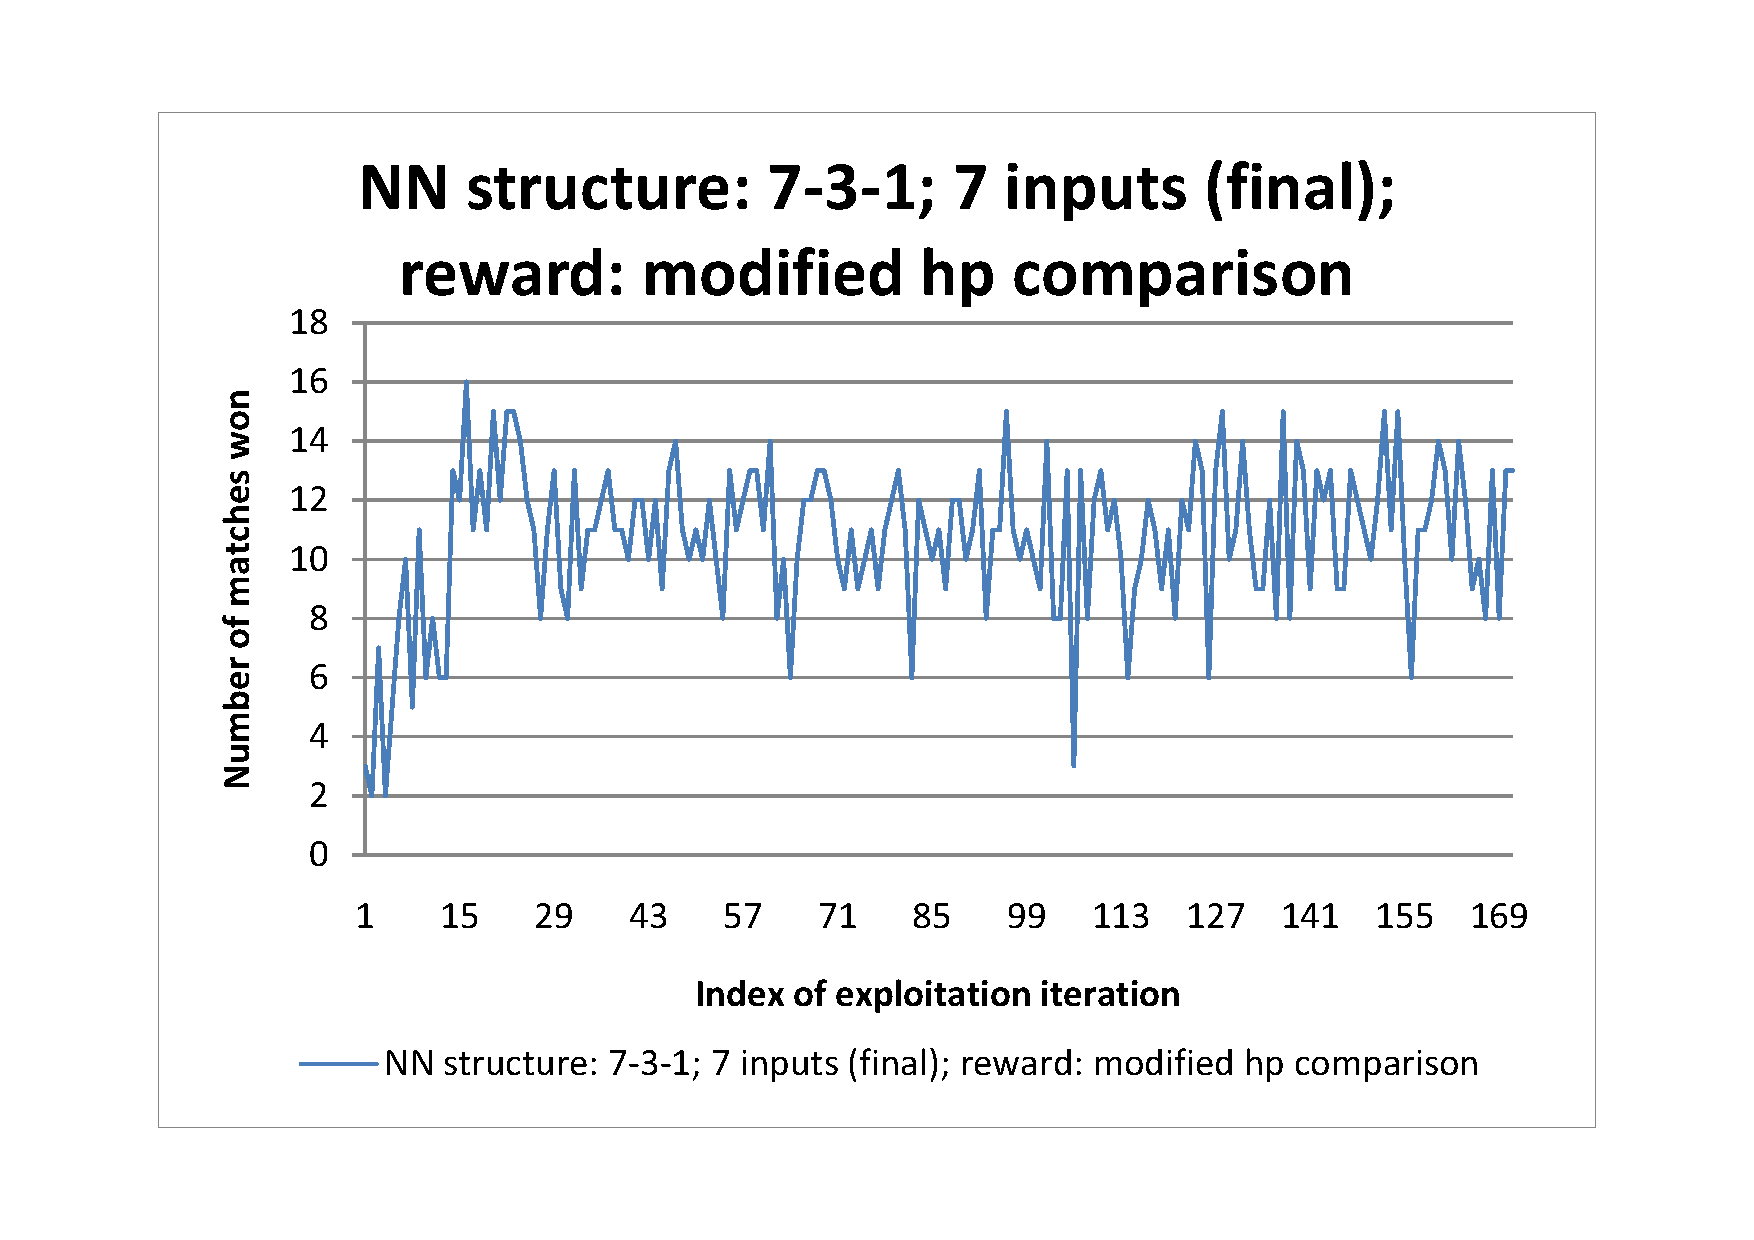
\includegraphics[width=1.0\columnwidth]{fig_ql_731_7(f)_r3_all}}
\caption{Results of test with neural network structure: 7in-3-1out}
\label{fig:nnfr}
\end{figure}
%%
\begin{figure}[htp]
\centerline{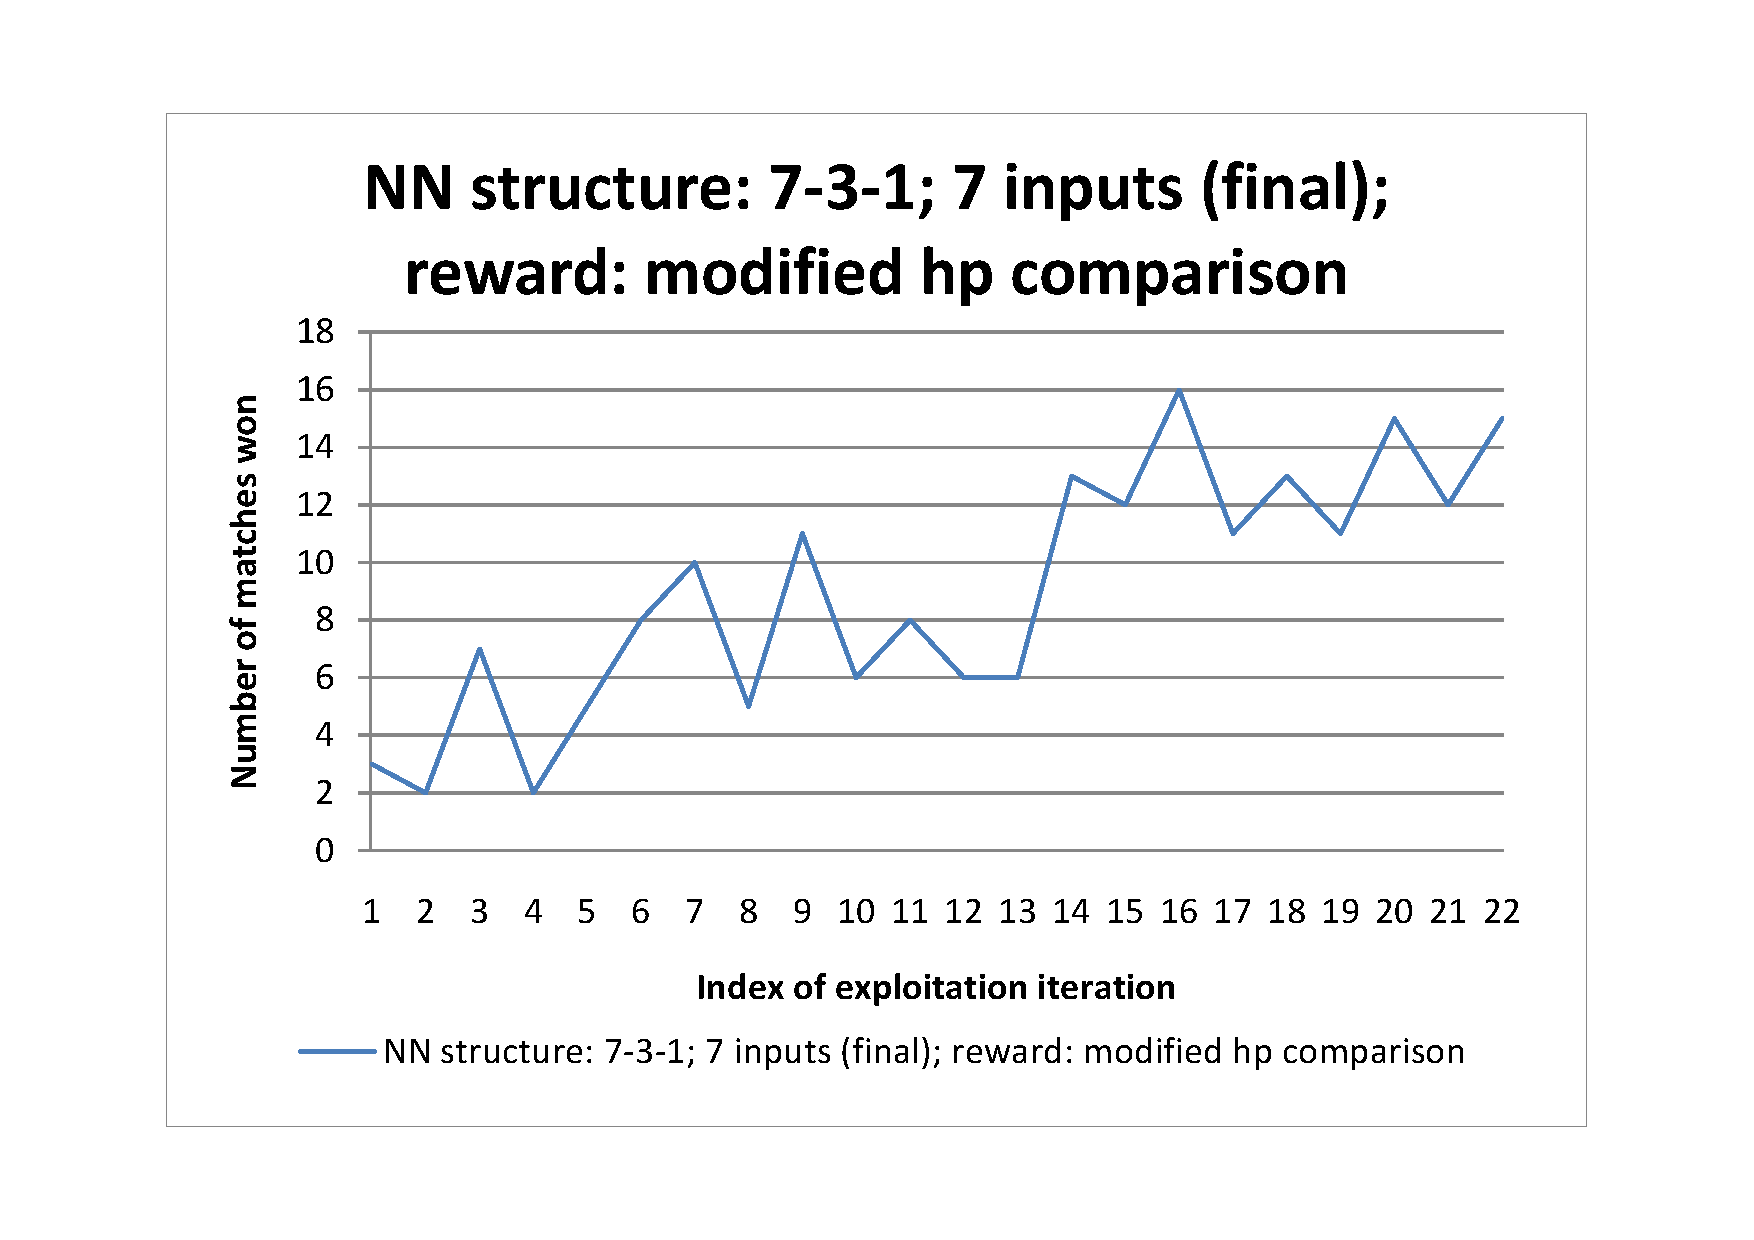
\includegraphics[width=1.0\columnwidth]{fig_ql_731_7(f)_r3_first20}}
\caption{First 22 iterations of results of test with neural network structure: 7in-3-1out}
\label{fig:nnff}
\end{figure}
%%
\hfill \\ \hphantom{x}
The strategy that bot learned was basically to move forward until enemy step inside bot unit weapon range and not to move during fire exchange. From algorithm point of view, bot learned that the best strategy is to give attack order.
\\ \hphantom{x}
Next tests were provided also for only one hidden layer, but with a different number of neurons in it in order to check it's impact on bot performance.
\\ \hphantom{x}
First of one hidden layer tests was test  with a neural network structure of 7 inputs, 7 neurons hidden layer and one output. The results of this test are presented on Fig.\ref{fig:nnt}. We can see that the results are a little unexpected. There is no visible learning process - at the beginning exploitation results are between 1 and 16 won matches, although with time they are tending to value of 9.
\begin{figure}[htp]
\centerline{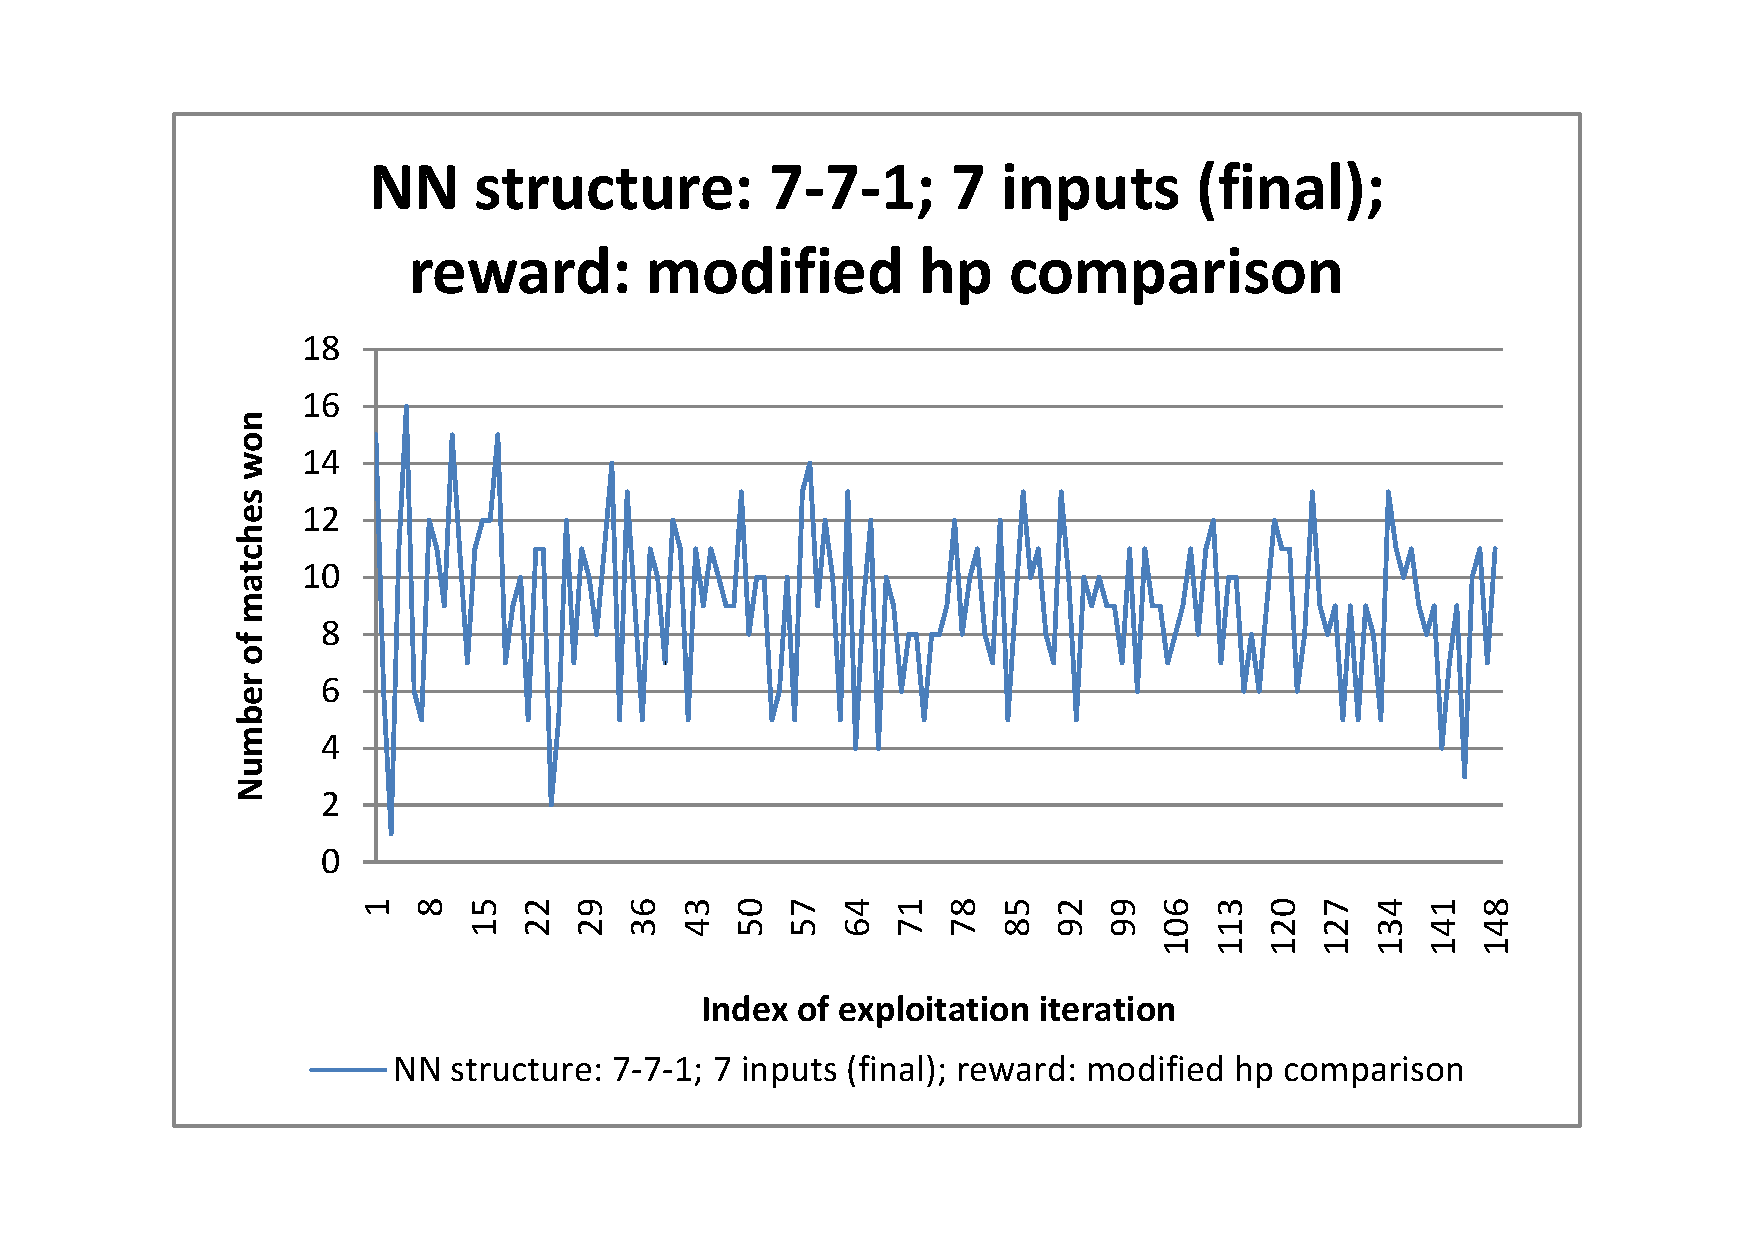
\includegraphics[width=1.0\columnwidth]{fig_ql_771_7(f)_r3}}
\caption{Results of test with neural network structure: 7in-7-1out}
\label{fig:nnt}
\end{figure}
%%
\hfill \\ \hphantom{x}
Again, bot came up with strategy to move forward and attack enemy as soon as he will step inside it's unit weapon range and not to move during fire exchange which is again a strategy to give attack order all the time.
\\ \hphantom{x}
Next test brought also a little unexpected results. The neural network with structure of 7 inputs, 1 neuron in middle layer and one output appeared also tend to value of 9 matches won in one iteration and also no learning process is visible. However in case of this neural network structure, learning process is very fast due to very simple structure - neural network contains only two neurons. \\ \hphantom{x}
The second surprising fact was that a bot with that small amount of neurons is able to get to learn a strategy that allows him to win matches. Basically the bot learned to wait for enemy to enter it's weapon range and than start to shoot and not to move during fire exchange. The interesting difference from previous bots is also the fact that this bot achieves this waiting strategy in different ways: one time he just wait at it's starting position for enemy bot, but other times he withdraws for some time and then wait for enemy.
\begin{figure}[htp]
\centerline{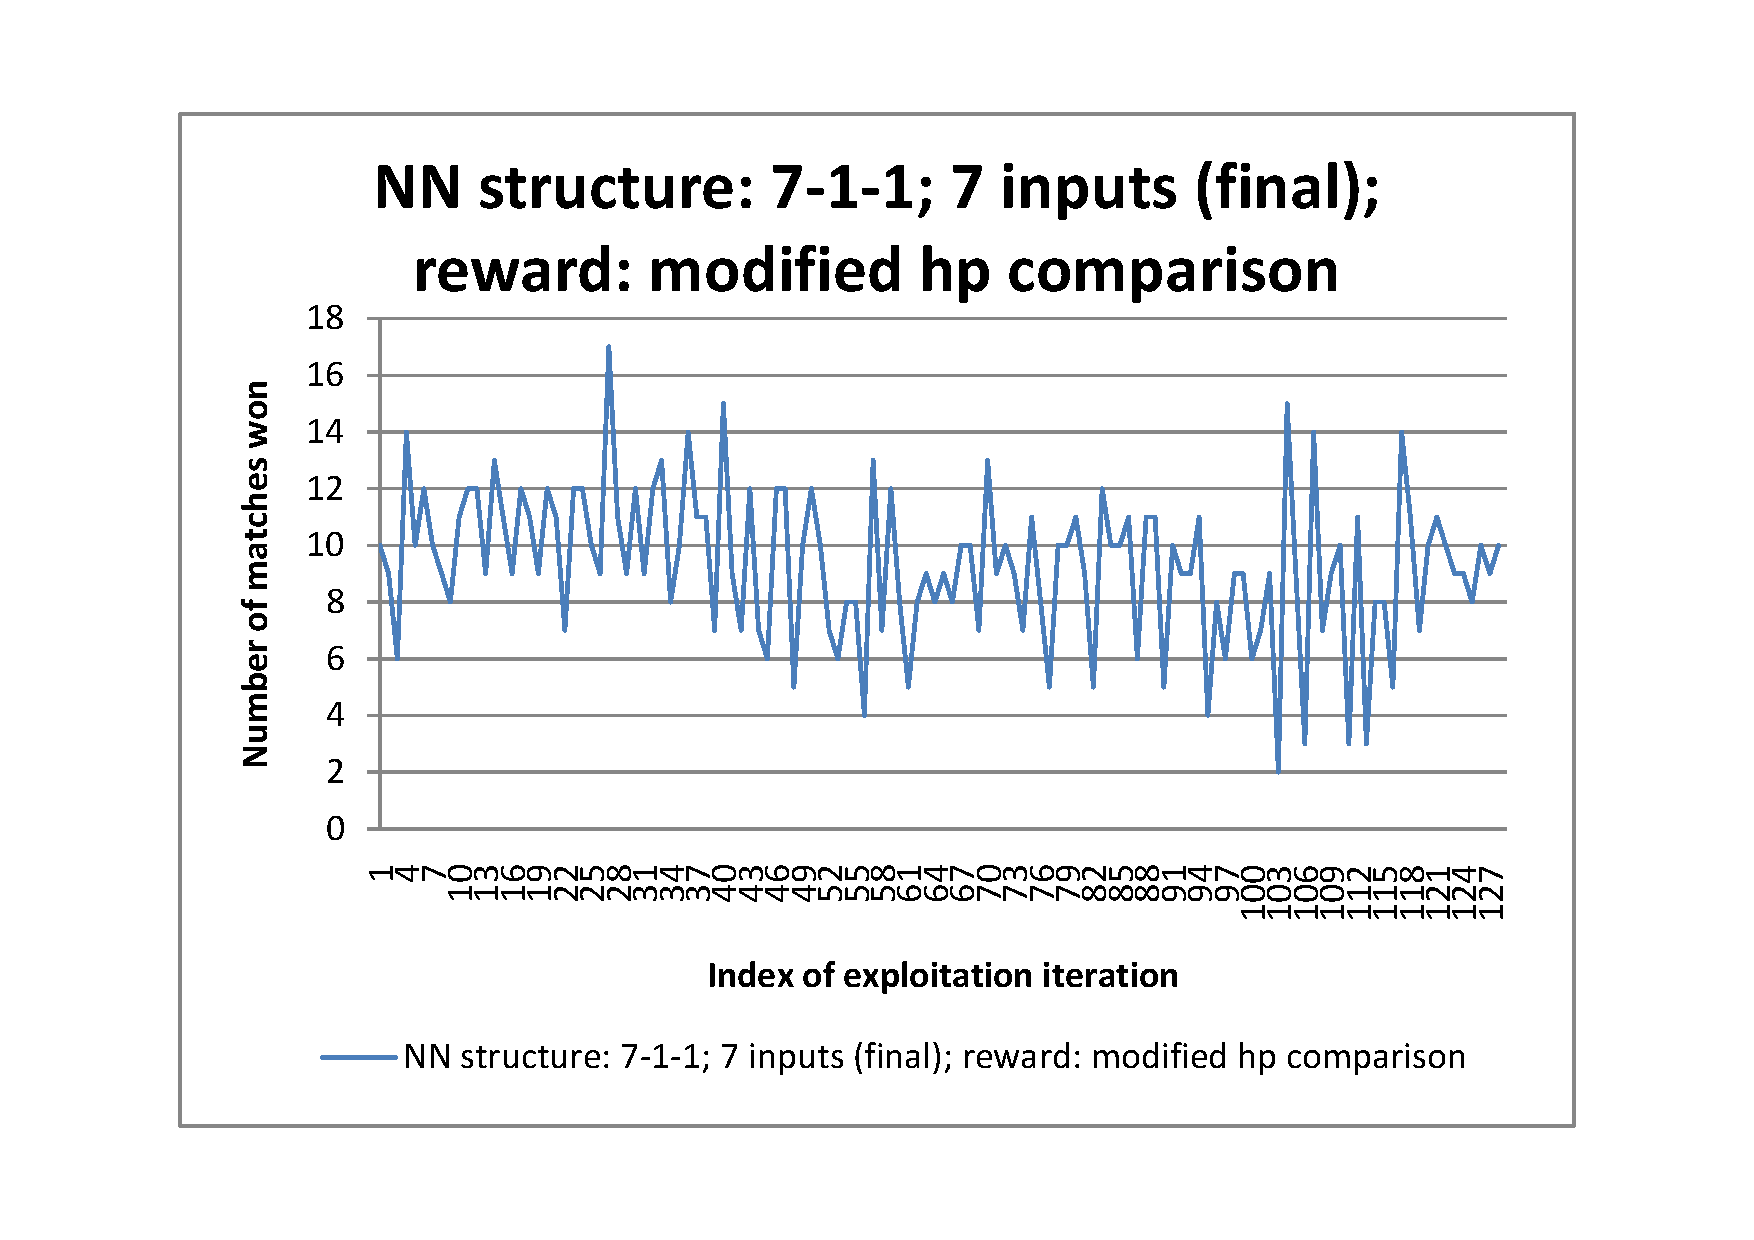
\includegraphics[width=1.0\columnwidth]{fig_ql_711_7(f)_r3}}
\caption{Results of test with neural network structure: 7in-1-1out}
\label{fig:nns}
\end{figure}
%%
\\ \hphantom{x}
At the end we also wanted to test bot with neural network of two hidden layer structure of 7 inputs, 3 neurons in first hidden layer, 2 neurons in second hidden layer and 1 output. The purpose of this test was to prove that adding more middle layers would not improve bot performance. The results are shown on Fig.\ref{fig:nnf} and allows us to see that bot starts to learn in approximately first 8 iterations and than it starts floating in range between 5 to 16 won games in iteration.
\begin{figure}[htp]
\centerline{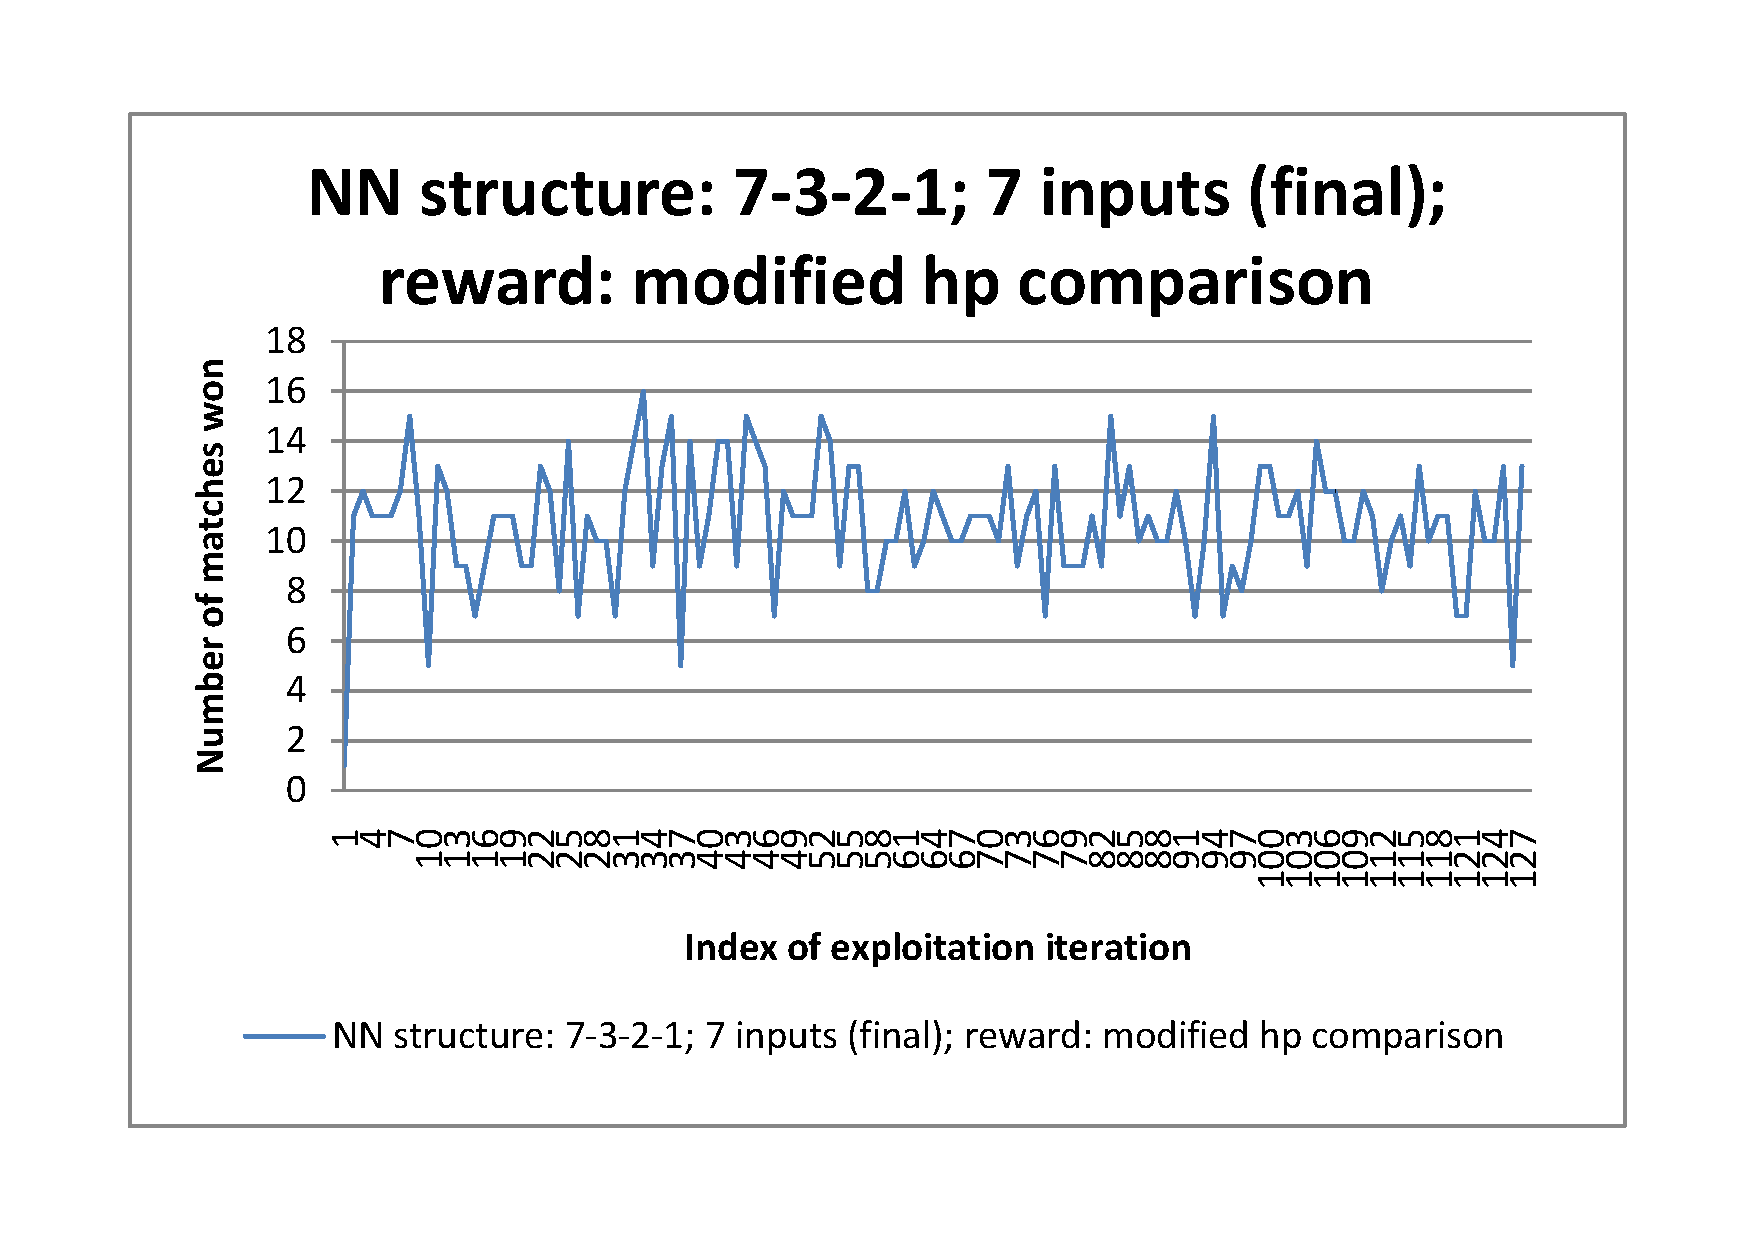
\includegraphics[width=1.0\columnwidth]{fig_ql_7321_7(f)_r3}}
\caption{Results of test with neural network structure: 7in-3-2-1out}
\label{fig:nnf}
\end{figure}
%%
\hfill \\ \hphantom{x}
The behavior of this last bot tested was similar to first two tested (bots 7-3-1 and 7-7-1).
\\ \\ \hphantom{x}
To summarize section about NN structure experiments, we would also like to discuss a floating aspect of all tests in this section. We discovered that game contain independent (in meaning that we do not have possibility to affect it) factor which affects match result.
\\ \hphantom{x}
This factor is an issue of who starts to shoot first. The problem is, that due to fact that both fighting units are of the same type, the unit who start to shoot first will definitely win the match. Theoretically there is 50\% chance for each unit to perform this operation first so this factor has a huge impact on match result.
\\ \hphantom{x}
From performed tests we can see that this factor is affecting about half of the games - all obtained results showed on line graphs indicates that the number of matches won in each iteration is floating around value of 10 which is half of all exploitation matches played in iteration.
%%%

%-------------------------------------------------------------------------------------------------------------------------------------------------
\subsection{T-tests} \hfill \\ \hphantom{x}
T-test were made in comparison to bot with structure of 7-3-1 for all other different neural network structure bots that were tested. We used two-tailed tests. Tests are based on amount of hit points left on board - at the end of a match bot unit hit points and enemy unit hit points are subtracted and normalized by greater of maximum fighting units hp value as it is shown at following formula:
\begin{IEEEeqnarray}{rCl}
hp\_left = \frac{uhp-ehp}{\max\{muhp,mehp\}},
\label{equation:reward}
\end{IEEEeqnarray} 
where:\\
uhp - unit hit points,\\
ehp - enemy unit hit points,\\
muhp - maximum unit hit points,\\
mehp - maximum enemy unit hit points.\\ \hphantom{x}
This formula provides output values in range from -1 to 1, where -1 is 100\% enemy unit hit points and 1 is 100\% bot unit hit points.
%
\\ \hphantom{x}
T-test results are shown in table \ref{table:ql_ttest}. Row $\mu$ is a sample mean value, row $\sigma$ is a sample standard deviation value, p-value can be found in $p$ row. The \emph{hypothesized mean} is a mean value for bot with 7-3-1 neural network structure (marked with a \emph{(ref)}) .
% ---------
\begin{table}
\caption{T-test values table}
\begin{center}
\begin{tabular}{|l|r|r|r|r|}
\hline
\multicolumn{1}{|c|}{\bf T-test } & 
\multicolumn{1}{|c|}{\bf 7-3-1 (ref) } & 
\multicolumn{1}{|c|}{\bf 7-1-1 } & 
\multicolumn{1}{|c|}{\bf 7-7-1 } & 
\multicolumn{1}{|c|}{\bf 7-3-2-1 } \\
\hline
{\it $\mu$} &          0.007501 &        -0.006933 &          -0,094653 &       0.004547 \\
\hline
{\it $\sigma$} &          0,112205 &      0,110452 &          0,224809 &          0.127824 \\
\hline
{\it $p-value$} &          - &       1.02 $\times$ 10$^{-10}$ &          8.106 $\times$ 10$^{-123}$ &          0.2442 \\
\hline
\end{tabular}  
\label{table:ql_ttest}
\end{center}
\end{table}
% ---------
%%%

%-------------------------------------------------------------------------------------------------------------------------------------------------
\subsection{Discussion} \hfill \\ \hphantom{x}
The results of different neural network structure bots compared in table \ref{table:ql_ttest} with a t-test allows us to see structure impact to bot's performance. Bots with structures of 7-7-1 and 7-1-1 appeared to be significantly worse than referenced bot. The null hypothesis is rejected with significance level of 1\%. Contrary to expectations, a two hidden layer bot appeared to be second best with the null hypothesis not rejected even with a significance value of 10\%. Based on mean values of \emph{hit points left on board}, the best neural network structure appeared to be first tested (7-3-1), but wen we take into account learning speed, unexpectedly a bot with two hidden layers is better with approximately 8 learning iterations while 7-3-1 bot needed approximately 16. \\ \hphantom{x}
%
During tests it occurred that the best tactic in order to win a match is to provide only attack decisions at least during the fire exchange. \\ \hphantom{x}
%
The biggest problems we found were during the first preliminary tests with both state representation and reward mechanism. It took us a long time to find final solution. First attempts of small value rewards during the match were unsuccessful - values were to small and also targets of rewards inaccurate. In state representation the most problematic input occurred to be distance between fighting units. We tried three different approaches before we found the right one. \\ \hphantom{x}
%
As for further improvements, our bot could be expanded in a way that would enable to provide fights between different kinds of units of all races. This expansion would require to include additional inputs connected with other than Terran units statistics as shield of Protoss units for example. However, the balance of Starcraft game is so well designed that most of one versus one unit fights are from top doomed to end in a certain way. For example zergling unit will always loose against marine unit and marine unit will always loose against zelot unit. Therefore the only purpose of modifying implemented QLeqrning bot would be for symmetrical fights. \\ \hphantom{x}
%%%

%
% INPUT
% everything related to Genetic Algorithm
% Main-Author: Prakash
%
%-------------------------------------------------------------------------------------------------------------------------------------------------
\section{Genetic Algorithm}
\label{section:GA}
%-------------------------------------------------------------------------------------------------------------------------------------------------
One of the drawbacks of using a Reinforcement Learning strategy is that the training schema can potentially lead to a localized solution space. Such a solution might not have evaluated all possible strategies. This drawback can be countered by using the robustness of methods such as Genetic Algorithms, which carry out more thorough search. We use such a method in order to evolve a Neural Network controller managing the bot in a 1 unit Vs 1 unit fight. This methodology is called \emph{Neuro Evolution} in general.

%-------------------------------------------------------------------------------------------------------------------------------------------------
\subsection{Representation} 
Our objective for the neural network is to be able to make informed decisions by interpreting the game state. Hence, a representation for the game state needs to be formulated. This representation needs to be minimal since the number of inputs to the neural network directly correlate to the size of the chromosome to be evolved. In this approach, we use 8 inputs, 4 for each unit involved in the combat: 
\begin{enumerate}
\item \emph{Shots to Death} - This heuristics utilizes the fact that all units in the game, at any given time, will be eliminated by a particular opponent unit in certain number of attack commands. This parameter can be used to represent several values at the same time - \emph{Hit-points}, \emph{Armor}, \emph{Opponent's Damage} and \emph{Damage Multiplier}, combined in equation:
\begin{equation}
\label{equation:nShots}
\text{shots}=\left \lceil\frac{\text{HP}}{(\text{damage}\times\text{times}-\text{armor}) \times\text{mul}} \right \rceil \text{,}
\end{equation}
This input is normalized over the maximum value of shots left to death when the game starts (maximum hot-points).
\item \emph{Distance} - This number signifies the distance of the unit from the opponent, which is normalized over its weapon range.
\item \emph{Cooldown Left} - The number of updates left before the unit can shoot again, which is normalized with the largest weapon cooldown time for the two units.
\item \emph{Speed} - The unit's top movement speed possible. This is again normalized by the maximum speed out of the two units.
\end{enumerate}
The neural network can provide 3 output values, each corresponding to an action's desirability ({\bf Move Towards Enemy}, {\bf Move Away from Enemy} or {\bf Attack}). The action with the maximum desirability is performed.

%-------------------------------------------------------------------------------------------------------------------------------------------------
\subsection{Algorithm Parameters}
\begin{enumerate}
\item \emph{Fitness}: The fitness of a particular chromosome is an integer value representing a Win ($1$) or a Loss ($-1$). To average out inaccuracy in fitness due to randomness, each chromosome is tested $20$ times and the fitness is averaged out. An alternate method to judge the fitness of a chromosome is to take an average of difference of hitpoints of the two units at the end of a match.
\item \emph{Choosing parents}: The natural selection method used in this project is Elite Selection. In a population of $N$ chromosomes, each reproduction cycle selects $\frac{N}{3}$ parents for breeding. However the selection method is modified in such a way that the chromosome with the best fitness is always selected (in order to not forget fitness comparison). The rest of the parents selected are uniformly distributed from the top portion of the population and bottom portion. This version is also comparable to the Roulette-Wheel selection methodology, where segments of the total population have certain selection probabilities.
\item \emph{Crossover}: The selected parents reproduce themselves by a simple one point crossover approach. The selection of the split point is normally distributed for each gene.
\item \emph{Mutation}: Each child gets mutated with a predefined mutation probability (standard value used in experiments is $0.2$). It is a recommended strategy to mutate a gene representing neural network connection weight by adding a Gaussian Random number. This enables the weight to be not bound within a particular range and enhance progression in the search space.
\item \emph{Population Refresh}: All newly produced children, two per parent (i.e. $\frac{N}{3}$ parents generate $\frac{N}{3}$ children), automatically replace the $\frac{N}{3}$ chromosomes at the bottom of the population (not replacing if a chromosome which was selected for parenting). The remaining $\frac{N}{3}$ part of the population is completely mutated, meaning that their each gene mutates with a probability of $1.0$.
\item \emph{Optimization}: Genetic Algorithms need a lot of fitness updates, especially in this case where a match to test fitness of a chromosome takes approximately 7 sec. Therefore one performance optimization made for the project is to preserve the fitness value of chromosomes that have not changed. In general, these are the chromosomes that were selected for parenting.
\end{enumerate}

%-------------------------------------------------------------------------------------------------------------------------------------------------
\subsection{Results} 
%%%

\begin{table}
\caption{average winning rate}
\begin{center}
% Table generated by Excel2LaTeX from sheet 'Sheet1'
\begin{tabular}{|r|r|r|r|}
\hline
       &       {\bf mean }&    {\bf stdev} &  {\bf p-value} \\
\hline
	\emph{8.8.4.3 (ref)} & $  0.025$ &  $ 0.099 $ &        --- \\
\hline
	\emph{ 8.8.3 }&   $0.019$ &  $  0.099 $ & $ 0.459 $ \\
\hline
 	\emph{8.1.3 }&  $ 0.014$ &   $ 0.104 $ & $ 0.094 $ \\
\hline
\end{tabular}  
\label{table:winningRate}
\end{center}
\end{table}
% ---------

\begin{enumerate}
\item Neural Network Structure - While designing the agent, one of the things on our mind was for the neural network to be able to process the inputs efficiently and try to decipher the optimal output values. But there is no way to understand the relation of the input values to the playing strategy for the agent. To test what structure of the neural network can achieve the most efficient results for the bot, we run T-tests with $3$ different structures of the network:
\begin{itemize}
\item Inputs (8), Hidden Layer (1), Output Layer (3)
\item Inputs (8), Hidden Layer (8), Output Layer (3)
\item Inputs (8), Hidden Layer (8), Hidden Layer (4), Output Layer (3)
\end{itemize}
The agent is trained in each case for a certain number of iterations (in this case they were trained for $60$ iterations) and then the best chromosome in each pool plays the game to create a sample space to be tested. The results for the T-test carried out on the three samples are presented in Table \ref{table:winningRate}. The samples are compared with respect to the $8,8,4,3$ network. While comparing the network with the $8,8,3$ neural network, the relatively high p-value signifies that they are similar. This means that the using the larger network is an overkill as it provides relatively similar output quality as the smaller network. This, however is not the case with the $8,1,3$ network. The low p-value means that the samples are not similar. Then the decision to select a network falls on the which has a higher success-rate (which is already being measured by the average fitness value of the chromosomes).
\begin{figure}[htp]
\centerline{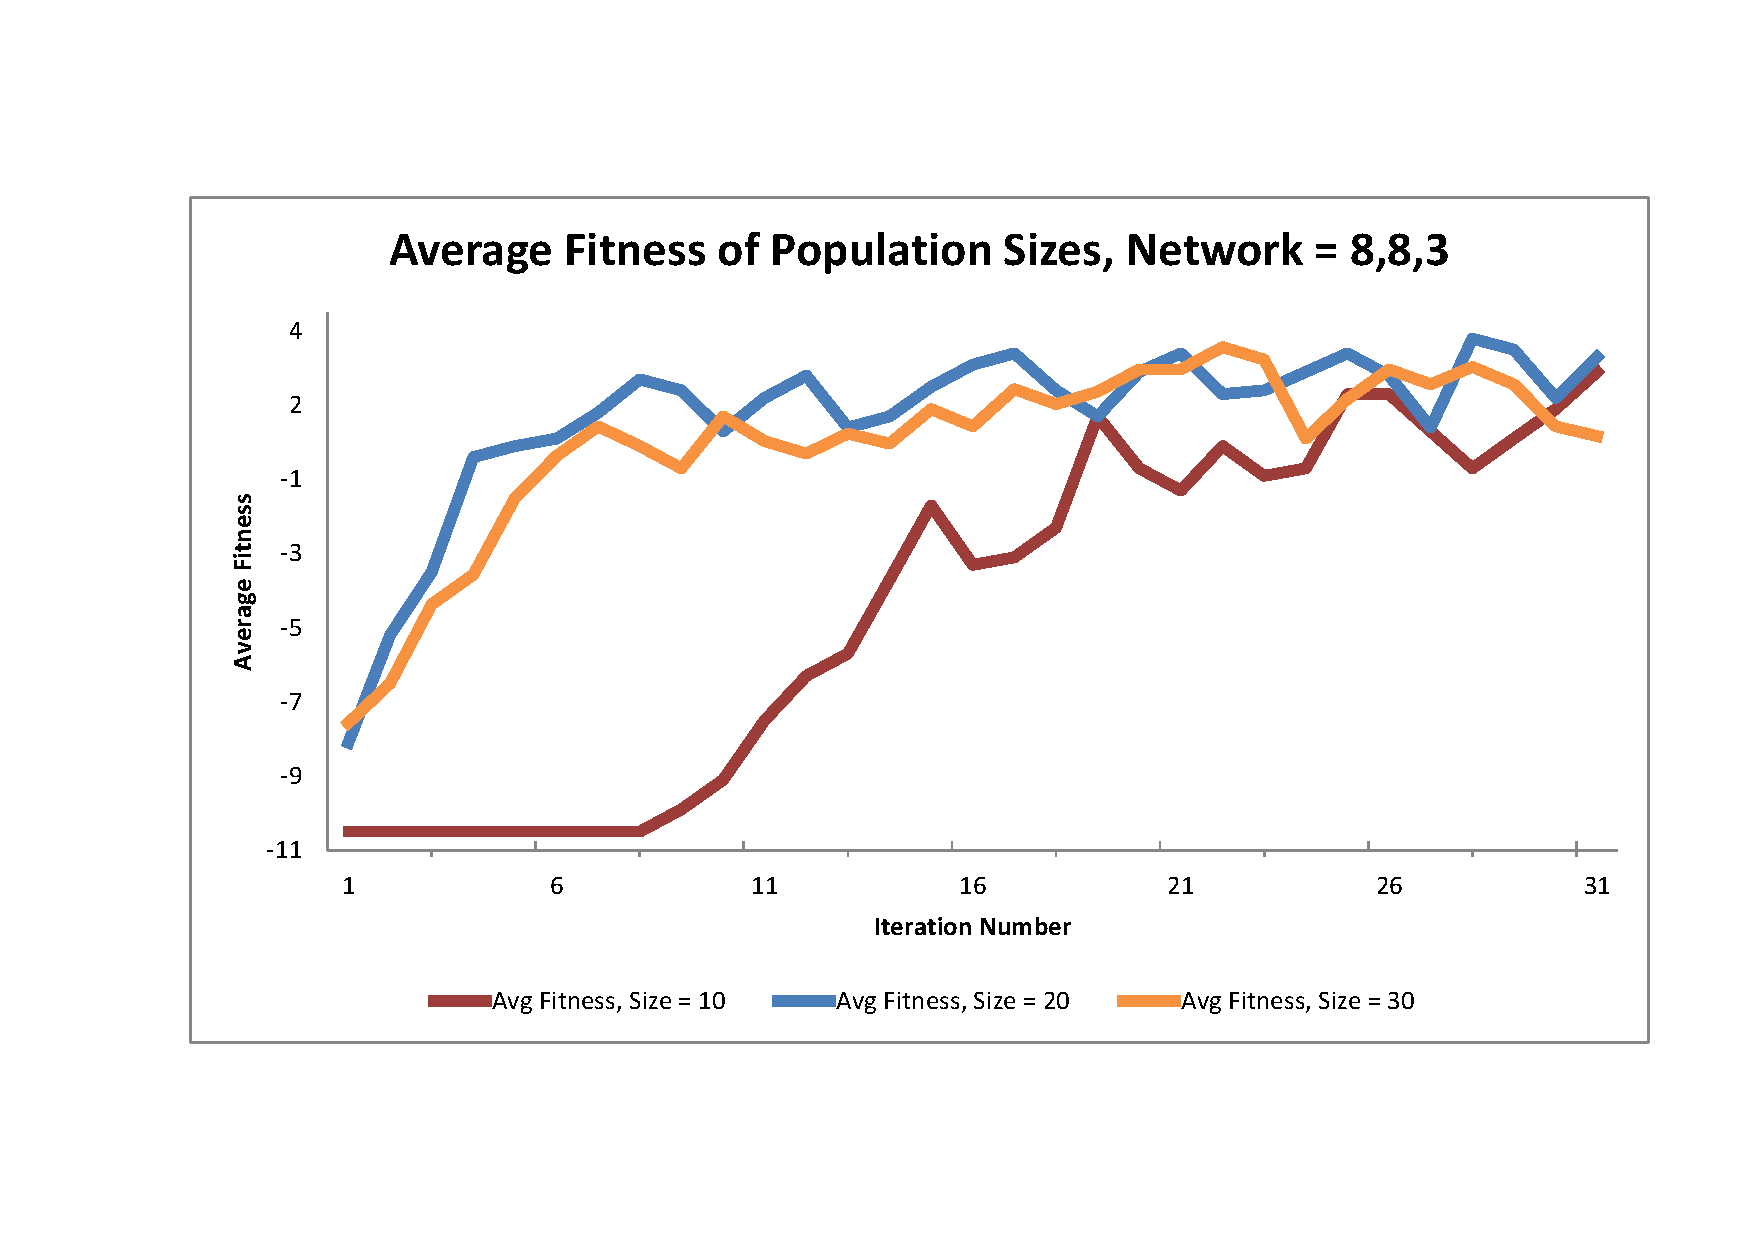
\includegraphics[width=1.0\columnwidth]{fig_GA_AverageFitness}}
\caption{Graph showing the progression of Average Fitness of population of size $10$, $20$ and $30$, respectively: NN configuration is $8,8,3$}
\label{fig:AverageFitness}
\end{figure}
\item Population Size - We are also interested in finding out the rate of convergence of the Genetic Algorithm, as well as its dependency on the population size. Generally a larger population size is preferred, since the high number of chromosomes provide a bigger search space for the algorithm to find a fit individual in. But this leads to a lot of overhead on the system to process individuals introduced on each iteration in the larger population. To assess this parameter, we look at a comparative Figure \ref{fig:AverageFitness} showing the progression of average fitness of the populations of sizes $10$, $20$ and $30$. The population with size 10 seems to be too small and has slow convergence to the other two populations. The other two populations are very close in average performance and hence a smaller and more efficient population size is selected. 
\begin{figure}[htp]
\centerline{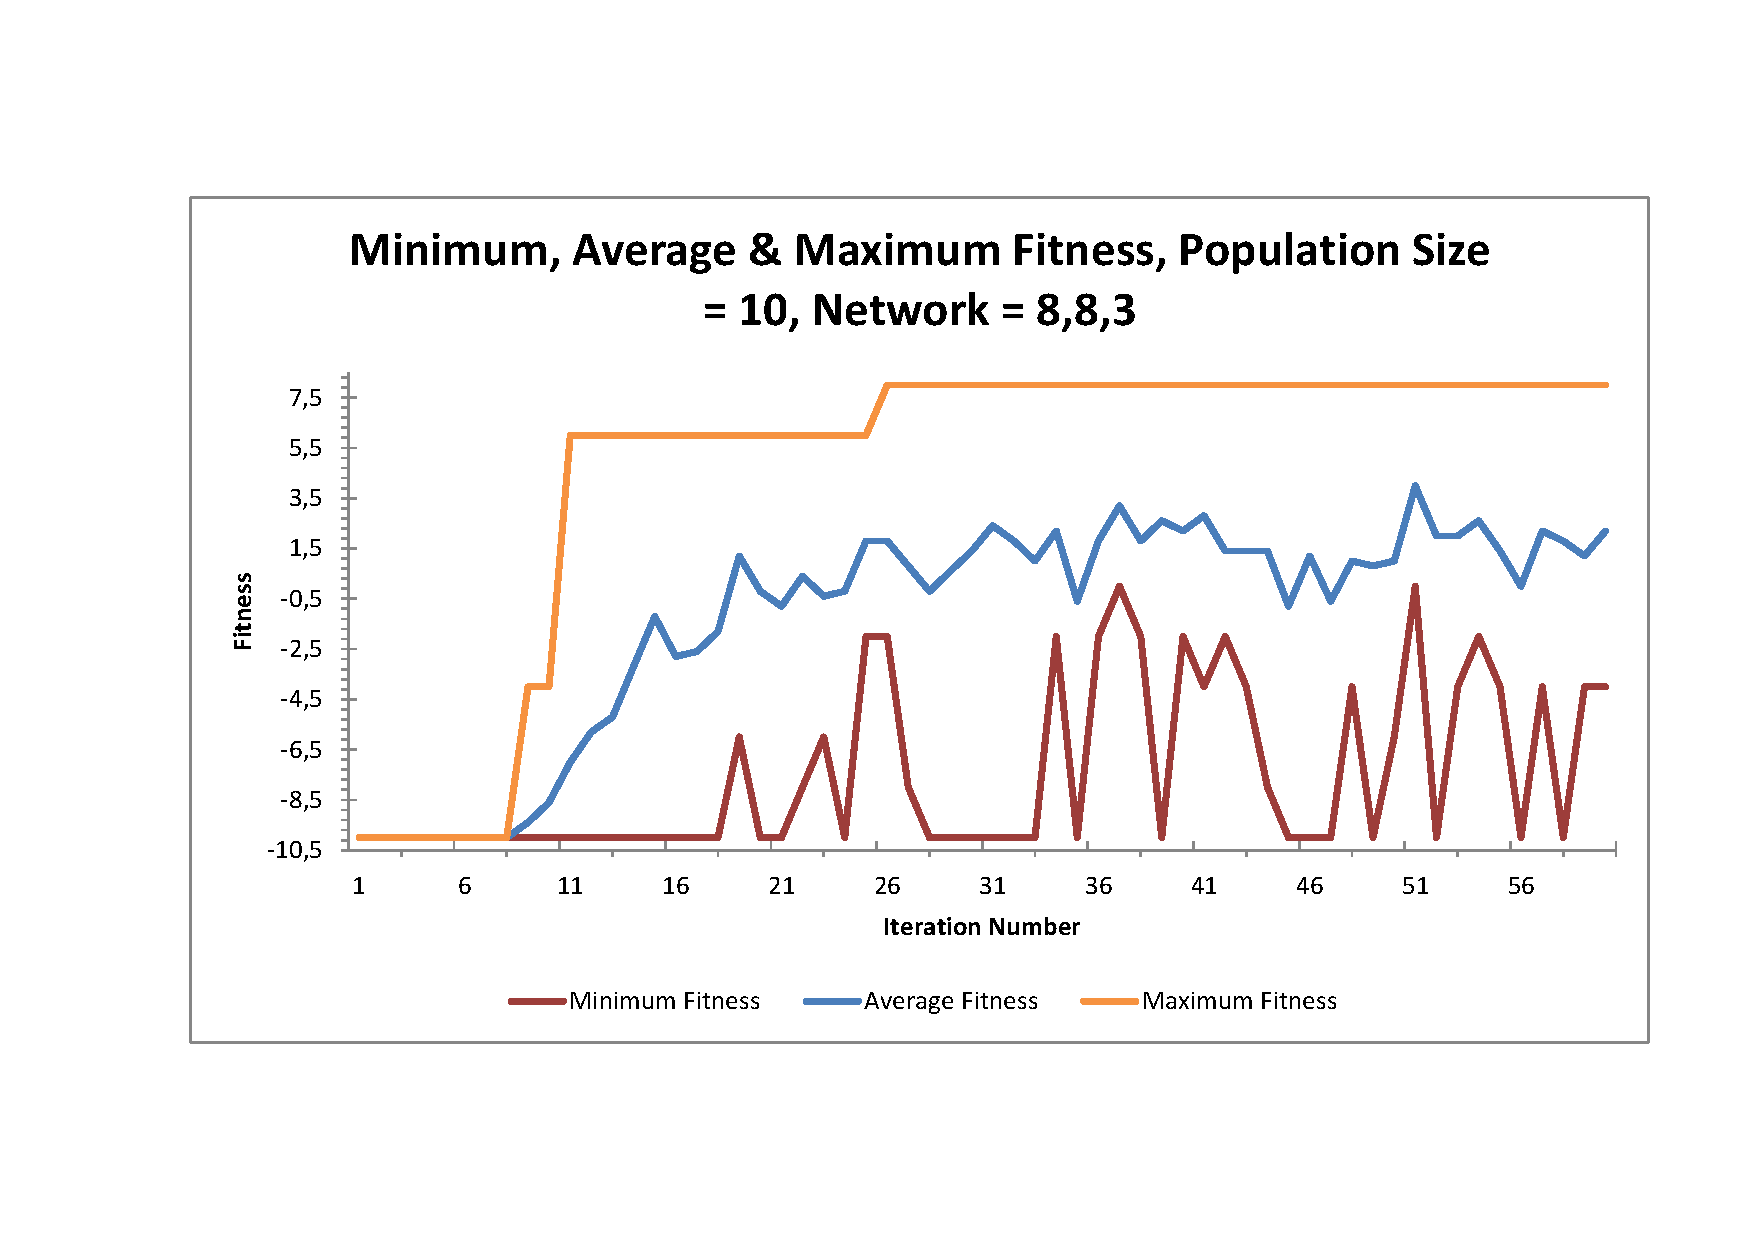
\includegraphics[width=1.0\columnwidth]{fig_GA_Fitness_MinAvgMax}}
\caption{Graph showing the minimum, average and maximum fitness of population of size $10$, NN configuration is $8,8,3$}
\label{fig:minAvgMaxFitness}
\end{figure}
\item Fitness Spread - In a genetic algorithm, the reproduction and discard rules are used to introduce new individuals to the population that can spread the solution in a much broader spectrum. This counters the problems provided by other computation intelligence algorithms to get stuck in local minima. A way to test the spread of the population is by graphing the minimum, average and maximum fitness of a population (size = $10$), as shown in Figure \ref{fig:minAvgMaxFitness}. A large distance between the minimum and maximum fitness points to the conclusion that the population is taking care of introducing diverse individuals.
\end{enumerate}

%%%
\begin{figure}[htp]
\centerline{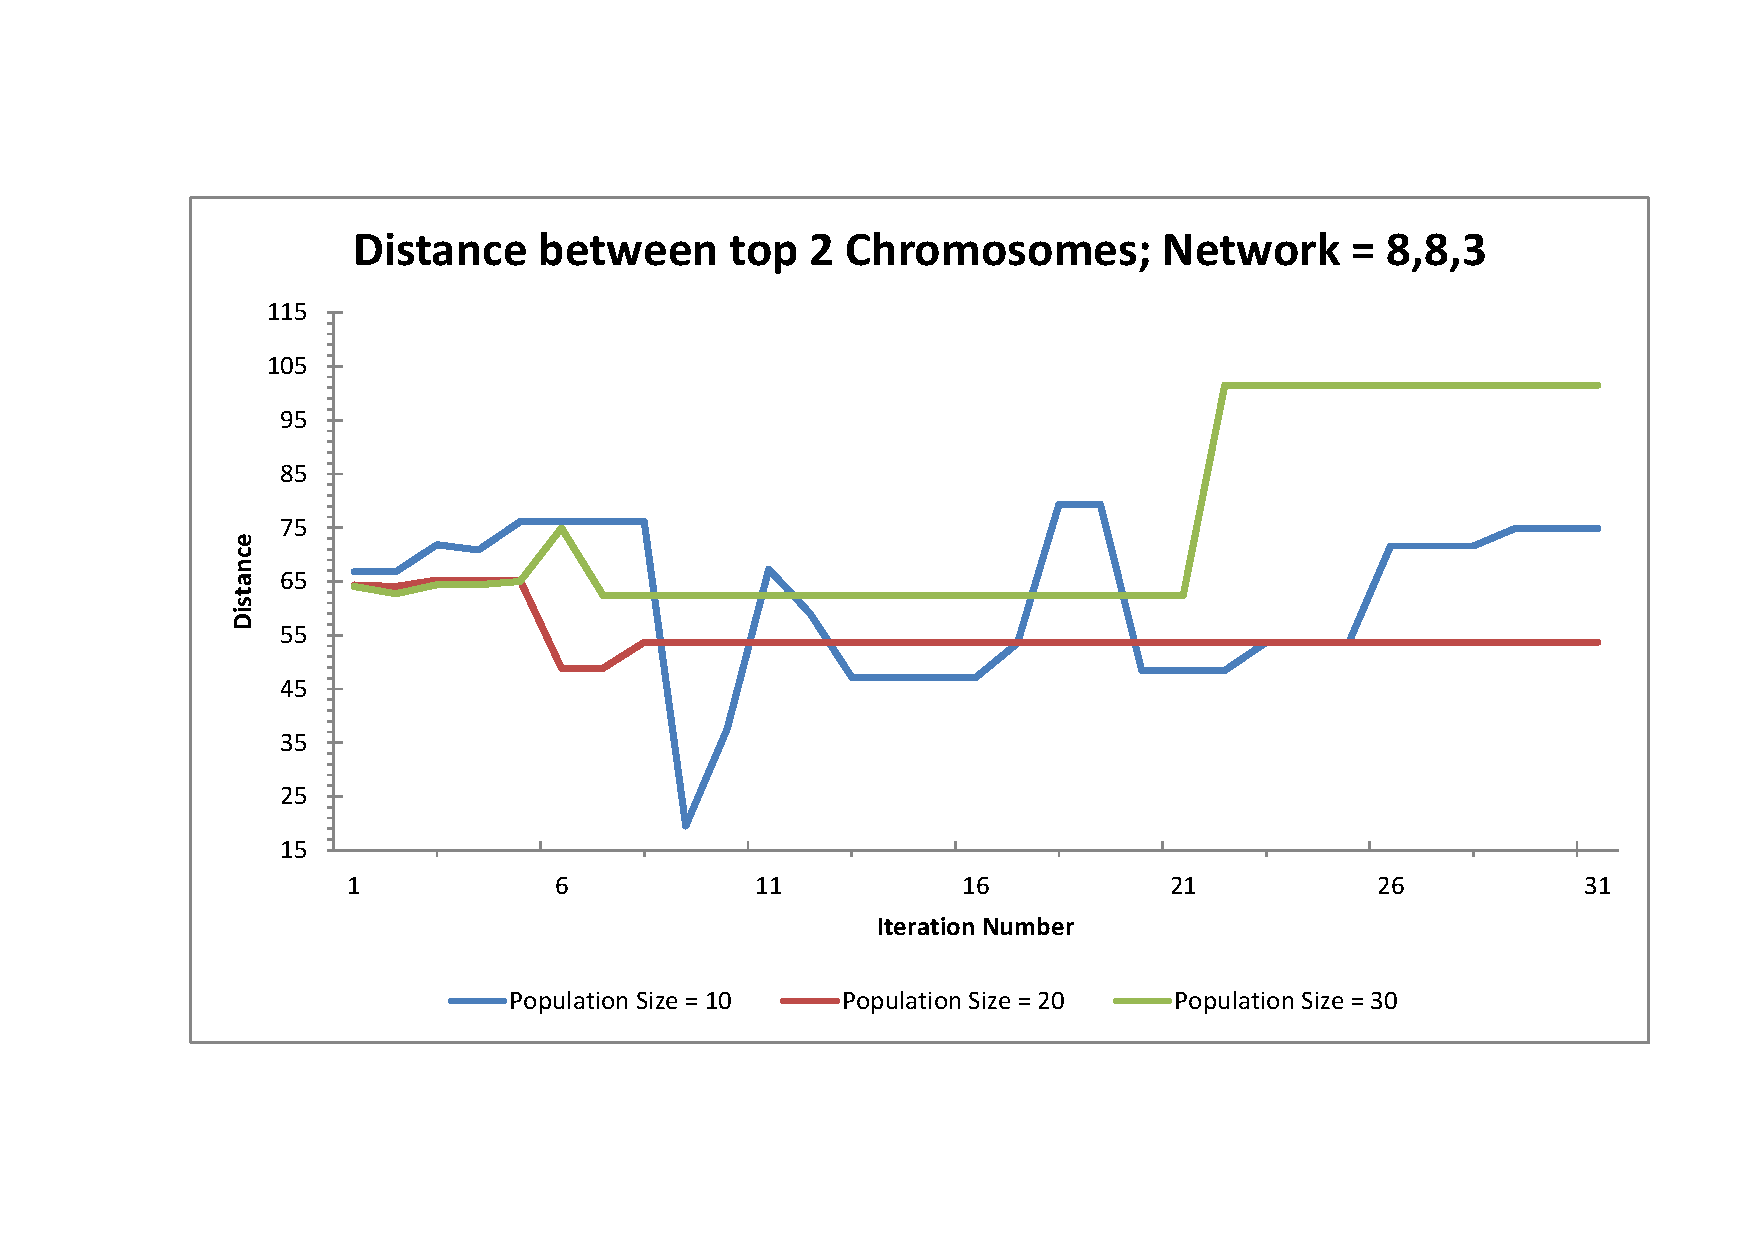
\includegraphics[width=1.0\columnwidth]{fig_GA_Speciation_Top2}}
\caption{Graph of Specie difference between the top two chromosomes}
\label{fig:specieTop2}
\end{figure}
\begin{figure}[htp]
\centerline{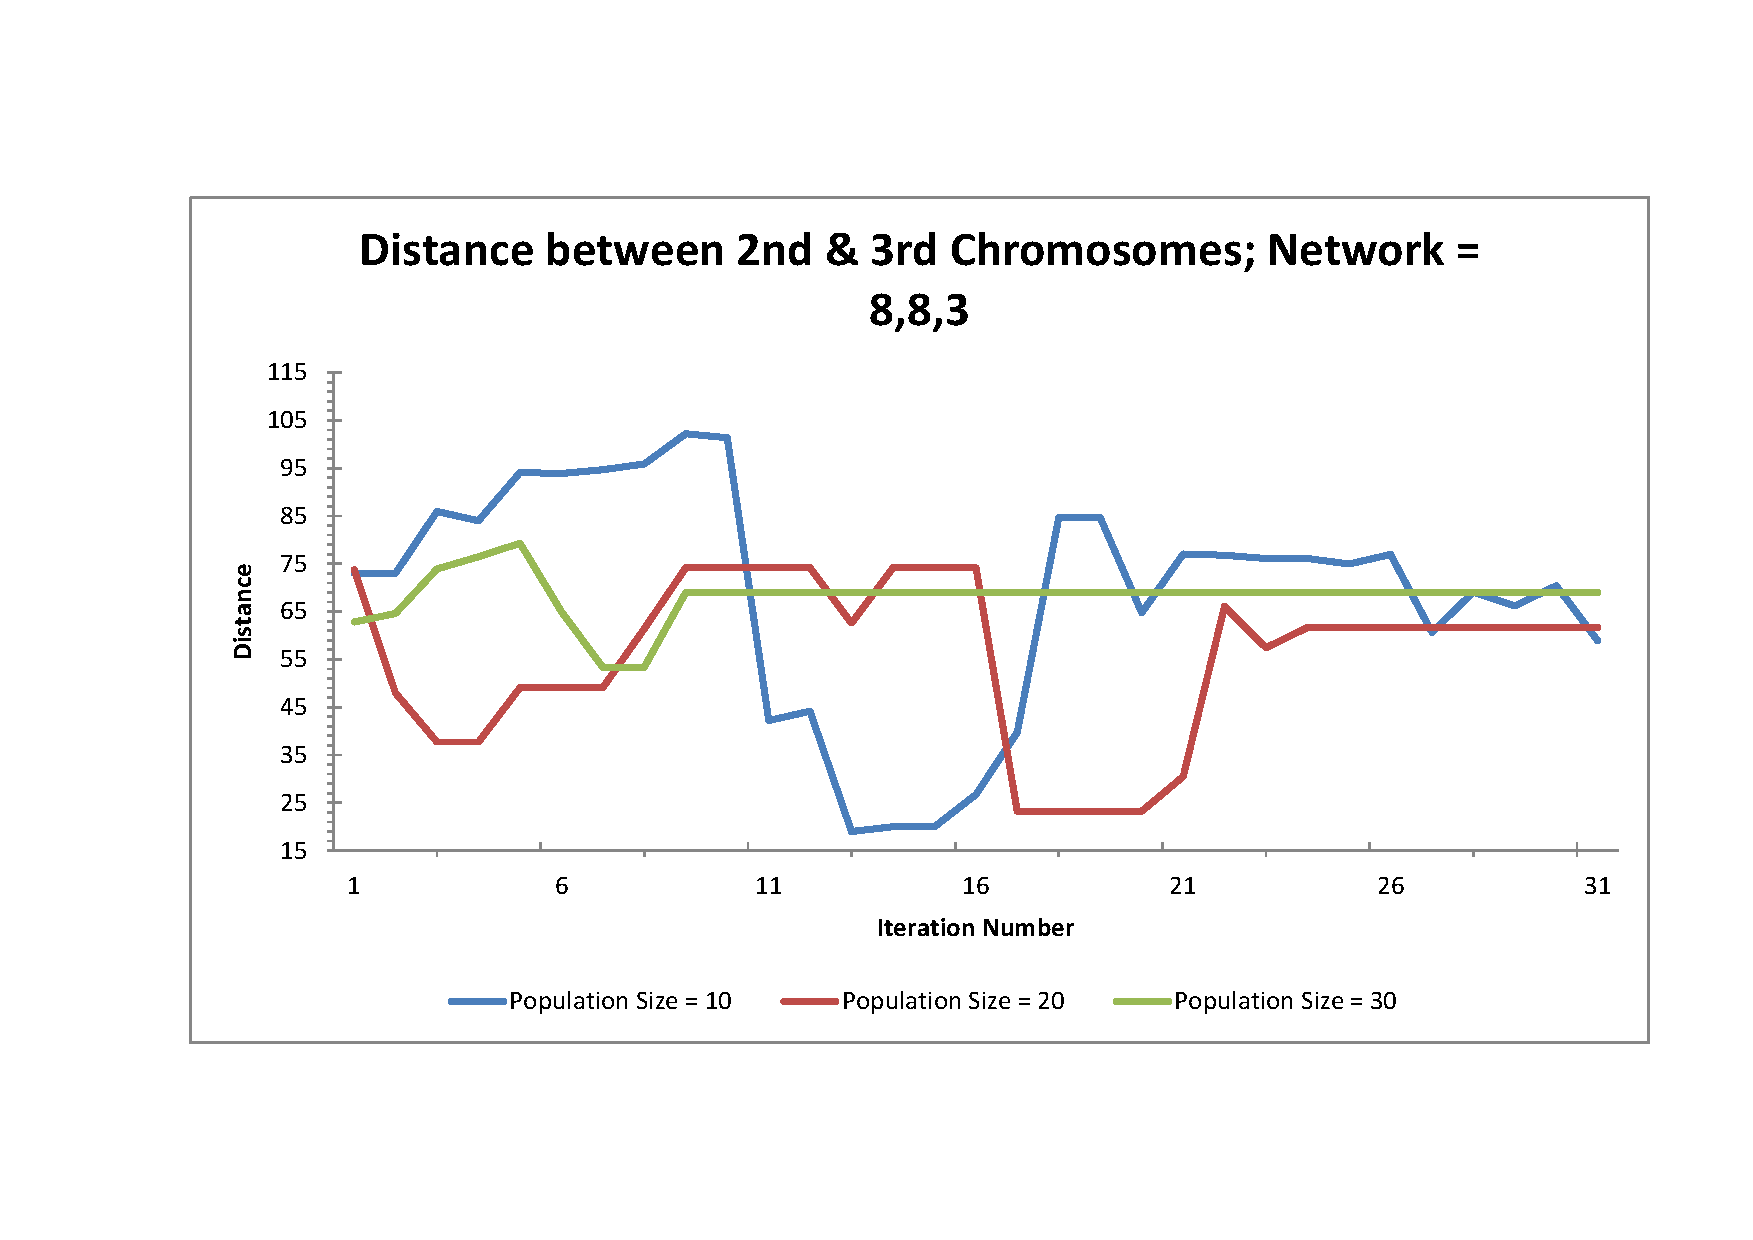
\includegraphics[width=1.0\columnwidth]{fig_GA_Speciation_next2}}
\caption{Graph of Specie difference between $2^{nd}$ and $3^{rd}$ ranked chromosomes}
\label{fig:specieNext2}
\end{figure}

%-------------------------------------------------------------------------------------------------------------------------------------------------
\subsection{Discussion}
According to our tests with the network structure and the population size, the best solution for our one versus one approach is a network structure of 8,8,3 and a population size of $20$. Although the bigger network also evolved well, in terms of performance we clearly have to choose the smaller one.
According to the figure \ref{fig:AverageFitness}, the population size of $20$, roughly scores as good as the population size of $30$. When we take the fact, that a smaller population size will evolve $\frac{1}{3}$ faster, into account, we have to chose a population size of $20$.

If we measure the cumulative distance between each gene of the top two candidates in the populations which is depicted in Figure \ref{fig:specieTop2}, we can see that the larger populations in genetic evolution hamper the evolving chances because of higher preservation of the top candidates. This can be attributes to the elite selection methodology we have employed that gives increasingly higher probability to the $1^{st}$ and $2^{nd}$ chromosomes to be selected for parenting.
This pattern becomes much more varied if we calculate the distance between the $2^{nd}$ and $3^{rd}$ chromosomes (Figure \ref{fig:specieNext2}), which depicts the higher chances for the chromosomes on those positions to be mutated.
%%%

%
% INPUT
% everything related to FuzzySystem
% Main-Author: David
%
%-------------------------------------------------------------------------------------------------------------------------------------------------
\section{Fuzzy System}
%-------------------------------------------------------------------------------------------------------------------------------------------------
\label{sec:fuzzy}
Our third approach for SC is a bot which performs small-scale combats on a flat terrain. The objective of this combat is to annihilate the opponent's units and the same amount and the same types of units are fighting against each other.
The decision-making of a unit is based on a Fuzzy Inference System.
%IMPLEMENTATION
The Fuzzy-System got implemented by our selfs and uses a stack for representing rules. The implementation got inspired by an open source AI framework called {\tt AForge.NET}\footnote{\url{http://code.google.com/p/aforge/}}.  %CITE to AForge?
%CITE to Game Programming Gems and lecture notes/slides
Further inspiration on how to use and implement fuzzy systems can be found in \cite{gpuGems2_fuzzy} and in our lecture notes.

In order to develop a squad control we decided to make the logic individuall for each unit. In contrast to GA or QL the unit performs strategies that suit group combats. Each unit decides on a individual basis and can perform the following actions:
\begin{description}
	\item[Attack:] \hfill \\
A unit performing this action attacks the enemy unit, with the lowest hit points.
	\item[Retreat:] \hfill \\
A retreating unit is moving away from the centroid of all enemy units.
\end{description}
The strategy of attacking the weakest unit is known to be effective in SC and is called \emph{focus fire}\footnote{\url{http://starcraft.wikia.com/wiki/Focus_fire}}. %
Due to the fact that lesser units cannot cause as much damage, this strategy tries to always kill the weakest. With weakest unit we mean the unit with the least amount of remaining hit points. The weakest one is also supposed to die fast resulting in a reduced enemy squad and less units able to attack our units. 

Our fuzzy logic tries to tackle this strategy by using a prevention system, which moves units, in danger to die, from the front-line to the back of our squad.

%REPRESENATION
%
%%FIGURE WITH THE RULES
%%%
\begin{figure*}[htbp]
\begin{center}
\begin{tabular}{ccc}
{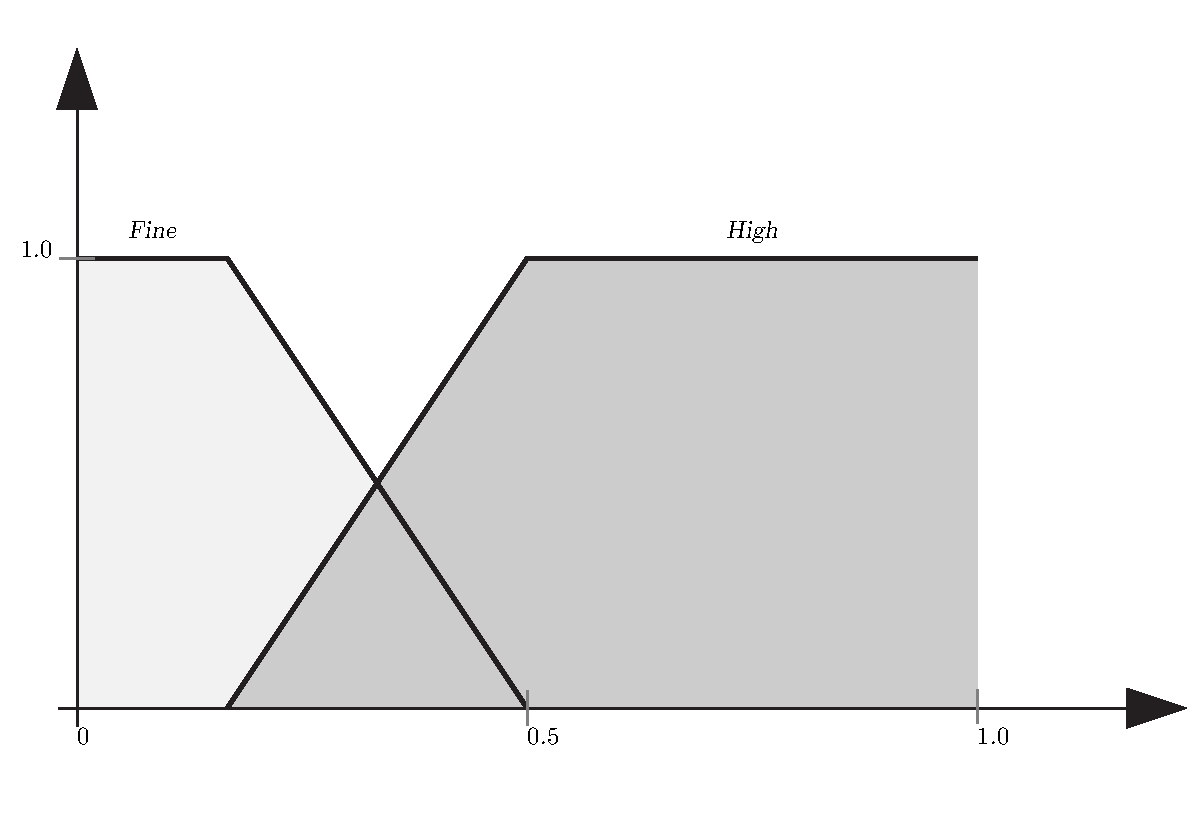
\includegraphics[width=1.0\columnwidth]{fig_fuzzy_deltaHealth}}&
{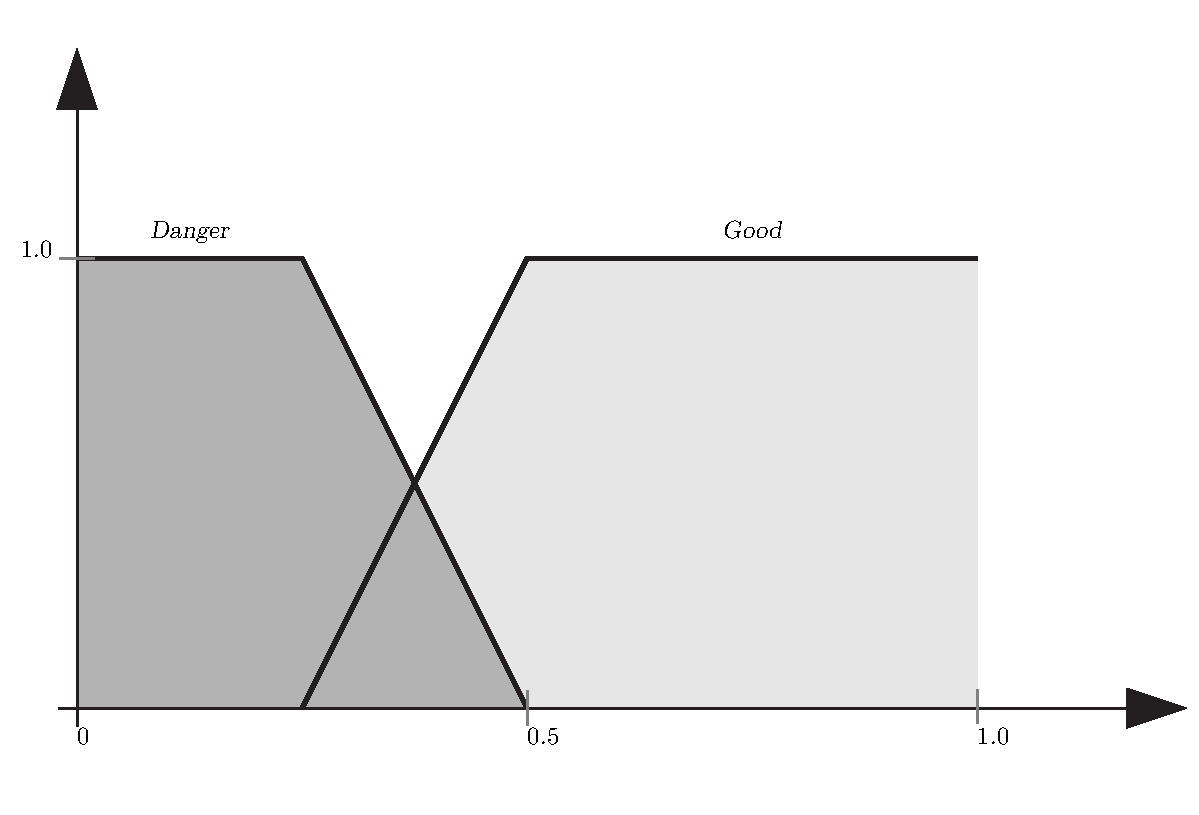
\includegraphics[width=1.0\columnwidth]{fig_fuzzy_health}}\\
{\it DeltaHealth } & {\it HitPoints }  \\
(a) & (b) \\
\end{tabular}
\end{center}
\caption{Linguistic variables and their fuzzy sets}
\label{fig:fuzzy_sets}
\end{figure*}
%
\begin{figure}
\begin{center}
\begin{tabular}{ccc}
{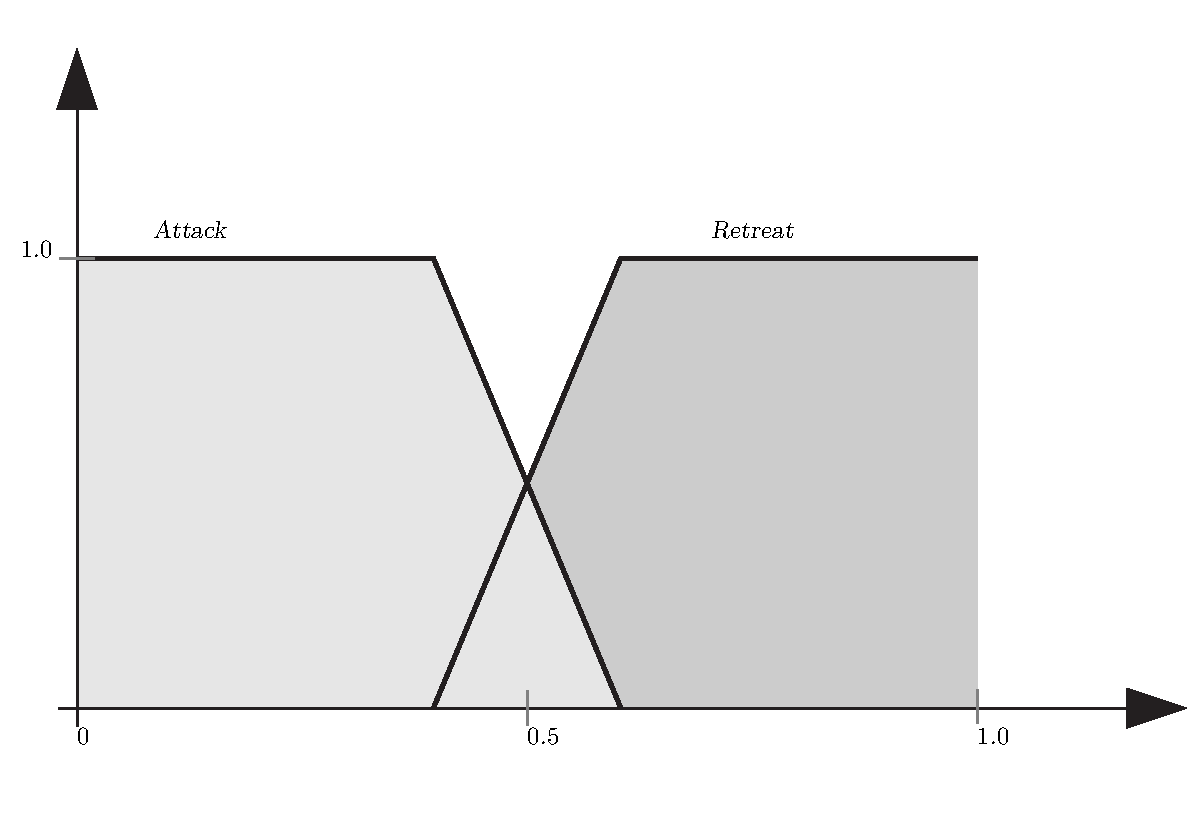
\includegraphics[width=1.0\columnwidth]{fig_fuzzy_stance}} \\ 
{\it Stance} \\
 (a) \\
\end{tabular}
\end{center}
\caption{Linguistic variable {\it Stance} and its fuzzy sets}
\label{fig:fuzzy_sets1}
\end{figure}
%%%
%%
%
For this approach we introduce three linguistic variables: {\it deltaHealth } ($\Delta \textrm{hP}$), {\it HitPoints } ($\textrm{hP}$) and {\it Stance}.
The fuzzy sets of the variables are as follows:
\begin{description}
	\item[{\it DeltaHealth:}] \hfill
	\begin{itemize}
		\item {\it Fine}
		\item {\it High}
	\end{itemize}
	\item[{\it HitPoints:}]  \hfill
	\begin{itemize}
		\item {\it Good}
		\item {\it Danger}
	\end{itemize}
	\item[{\it Stance:}]  \hfill
		\begin{itemize}
		\item {\it Attack}
		\item {\it Retreat}
	\end{itemize}
\end{description}

For a better overview the Figures \ref{fig:fuzzy_sets}(a), (b) and figure \ref{fig:fuzzy_sets1}(a) show the plotted fuzzy sets. The particular values of the fuzzy set get discussed later because we run some tests differing them. The range of all three variables is from $0.0$ to $1.0$. If a variable gets set above or below this range the values get clamped.

% Normalization of Inputs
Due to the fact that {\it DeltaHealth} only rises one frame, directly after we got hit by an enemy the impact of it would be only a short term one. To extend the range of one high hit, we calculate the {\it DeltaHealth} ($\Delta \textrm{hP}_i$) at a certain frame $i$ the following way:
\begin{align}
	\Delta \textrm{hP}_i &= \frac{( \textrm{hP}_{i-1} - \textrm{hP}_i ) + \Delta \textrm{hP}_{i-1}}{2}  \text{,}
\end{align}
where $\textrm{hP}_{i}$ is the {\it HitPoints} at the frame $i$. Before providing those values to the system they get normalized in the following way:
\begin{align}
	\textrm{inputDeltaHP}_i 	&= \frac{\Delta \textrm{hP}_i}{ \textrm{hP}_i} \\
 	\textrm{inputHP}_i 	&= \frac{\textrm{hP}_i}{ \textrm{maxHP}}  \text{,}
\end{align}
where $\textrm{inputDeltaHP}_i$, $\textrm{inputDeltaHP}_i$ are the inputs at frame $i$ and $ \textrm{maxHP}$ is the unit's initial amount of {\it HitPoints}.


With those fuzzy sets and variables we compose the following fuzzy rules:
\begin{enumerate}
	\item {\sl IF DeltaHealth IS High AND Health IS Danger THEN Stance IS Retreat }
	\item {\sl IF Health IS NOT Danger THEN Stance IS Attack }
\end{enumerate}

% :D ... fancy graph of the upper equations, maybe? :D

We applied our fuzzy set on different types of squad formations and we also differed the parameters for the fuzzy sets. Currently we only use the fuzzy sets {\it deltaHealth - High} and {\it HitPoints - Danger}. Due to that fact we don't talk about values for the other sets.
For our first test set, we call it \emph{fuzzy set 1}, we set {\it DeltaHealth - High} to the values $0.2$ and $0.5$. As shown in Figure \ref{fig:fuzzy_sets} this is a trapezoidal set which starts to rise from $0.2$ until it reaches the maximum at $0.5$ and stays at the maximum.
{\it HitPoints - Danger} got set to $0.3$ and $0.5$ which means the trapezoid starts with the maximum output at $0.0$ and falls in the range of $0.3$ to $0.5$ to a zero output.
Another test set (\emph{fuzzy set 2}) keeps the structure of  \emph{fuzzy set 1} and just moves the edges of the trapezoids.  {\it DeltaHealth - High} is  $0.00001$ and $0.1$ and {\it HitPoints - Danger} is set to $0.9$ and $0.99$.
\emph{Fuzzy set 3} sets {\it DeltaHealth - High} to $0.0001$ and $0.05$ and setting the fuzzy set {\it HitPoints - Danger} to $0.4$ and $0.5$.

The variable {\it Stance} stays the same for all tests and its fuzzy sets are trapezoidal shaped and are basically mirrored at the mid point ($0.5$). The {\it Attack} set covers the left half of the variable range with the values $0.4$ and $0.6$. {\it Retreat} also has the anchor points at $0.4$ and $0.6$, but this set covers the right half. Figure \ref{fig:fuzzy_sets1} (a) shows this set.

%LINGUISTIC VARIABLE AND IT'S MAPPING

%
\subsection{Results}
%-------------------------------------------------------------------------------------------------------------------------------------------------
%%%
\label{subsection:fuzzy:results}
%
Although the mechanics in SC are deterministic (especially weapon range and damage), the standard SC bot against whom our bot has to compete, makes random decisions. Therefore we have to run more games and average them. Most results in this section are the findings over a period of 100 games.
%
%%
\begin{table*}[htbp]
\caption{Fuzzy Logic: 2 Goliaths and 3 Marines Vs. 2 Goliaths and 3 Marines}
\begin{center}
\begin{tabular}{|l|r|c|c|c|c|c|c|c|ccccc}
\hline
	&  & \multicolumn{3}{|c|}{\bf summed HitPoints} 	& \multicolumn{3}{|c|}{\bf remaining units}  \\
	& \multicolumn{1}{|c|}{\bf lost} & $\mu$ & $\sigma$ & $p$ & 		$\mu$ & $\sigma$ & $p$ \\
\hline
{\it attacking (ref)}			&$ 1   $&$ 	176.12 $&$  48.52$&$ - $&$			2.63 $&$   0.87 $&$ - $ \\ %onlyAttacking.xlsx
\emph{ fuzzy set 1} 		&$ 2   $&$ 	153.61$&$   54.17$&$ 0.00 $&$ 			2.29 $&$   0.94 $&$ 0.00 $\\ %slighlyRetreating
\emph{ fuzzy set 2}		&$ 12 $&$ 	134.15 $&$  77.17$&$ 0.00 $&$     		2.15 $&$   1.13 $&$ 0.00 $ \\ %alwayRetreatingFuzzy.xlsx
\emph{ fuzzy set 3}		&$ 0 $&$ 	173.02 $&$  52.81$&$ 0.56 $&$     		2.59 $&$   0.85 $&$ 0.64 $ \\ %fuzzySet3.xlsx
%														not rejected at all
\hline
\end{tabular}  
\label{table:fuzzy_tTestSmallSquad}
\end{center}
\end{table*}
%%
%
Our initial tests with our three fuzzy set configurations are shown in Table \ref{table:fuzzy_tTestSmallSquad}. The squad for testing are 3 {\it marines} and 2 {\it goliaths} versus the same squad.
The table shows the average ($\mu$) and the standard deviation ($\sigma$) of the summed {\it HitPoints} and of our remaining units, for 100 games. The column \emph{lost} shows the amount of times the bot has lost out of this 100 games. As a reference we use a logic which is only attacking the weakest unit an never redrawing.
Initially there have been $5$ units and the initial sum of {\it HitPoints} is $370$.  The $p$-values can be found in the column $p$ and represent the results of a two-tailed test. 
%
%%
\begin{table*}[htbp]
\caption{Fuzzy Logic: 8 Goliaths Vs. 8 Goliaths}
\begin{center}
\begin{tabular}{|l|r|c|c|c|c|c|c|c|c|c|c|ccccc}
\hline
	&  & \multicolumn{3}{|c|}{\bf summed HitPoints} 	& \multicolumn{3}{|c|}{\bf remaining units}  &  \multicolumn{3}{|c|}{\bf frames per game}  \\
	& \multicolumn{1}{|c|}{\bf lost} & $\mu$ & $\sigma$ & $p$ & 		$\mu$ & $\sigma$ & $p$  & 	$\mu$ & $\sigma$ & $p$\\
\hline
{\it attacking (ref)}	&$ 1 $&$ 375.41 $&$   	126.88 $&$ - $&$			5.00 $&$   1.30 $&$ - $&$	 	415.61 $&$ 66.47  $&$ - $\\
\emph{ fuzzy set 3 }		&$ 4 $&$ 363.68 $&$    	152.92$&$ 0.44 $&$     		5.23 $&$   1.70 $&$ 0.18 $&$ 	427.54 $&$ 82.79 $&$ 0.15 $\\
\emph{ fuzzy set 3 (cleaned)} 	&$ 0 $&$ 380.30 $&$ 	136.29$&$ 0.72 $&$ 		5.48 $&$   1.36 $&$ 0.00  $&$ 	419.79 $&$ 76.11 $&$ 0.58 $\\
%								not rejected at all			rejected at 10 % significance level		rejected at 10% significance
%								not rejected at all			rejected at 1,5 and 10% significane level	not rejected at all
\hline
\end{tabular}  
\label{table:fuzzy_tTestBigSquad}
\end{center}
\end{table*}
%%
%
When this fuzzy logic gets applied to a different squad toplogy like eight {\it goliaths} versus eight {\it goliaths} it performs as shown in Table \ref{table:fuzzy_tTestBigSquad}. The table shows the average ($\mu$) and the standard deviation ($\sigma$) of the summed {\it HitPoints}, of our remaining units and the lost count of 100 games. The initial number of HitPoints when a game starts is $1000$ and there have been $8$ initial units. As a reference we use a simple logic which is only attacking the weakest unit an never redrawing. With a t-test we can show that some results are significantly better than the reference. The $p$-values can be found in Table \ref{table:fuzzy_tTestBigSquad} under the column $p$ and represent the results of a two-tailed test. 
The row {\it fuzzy set 3 (cleaned)} shows the data set when the $4$ lost games got removed.

%
\subsection{Discussion}
%-------------------------------------------------------------------------------------------------------------------------------------------------
%%%
The results of our test with the {\it marines} and {\it goliath} squad presented in Table \ref{table:fuzzy_tTestSmallSquad}, show that changing the fuzzy sets has an impact on the performance of our squad bot in the game. \emph{Fuzzy set 1} and \emph{ fuzzy set 2} are significantly worse than the simple attacking bot, in preserving HitPoints and in keeping units alive. The null hypothesis of the t-test gets rejected with a significance level of $1\%$.
The \emph{fuzzy set 3} bot seems better balanced and it cannot be shown that it is performing better or worse than the reference bot.
The bad performance of the \emph{ fuzzy set 2} bot can be explained by its behavior. It is retreating after every hit it takes and therefore gets more inefficient when the squad is decreasing, due to deaths of own units. The bot has no information about the squad-size and also withdraws even if there is only one unit left.
\emph{ Fuzzy set 1} is not as bad as \emph{ fuzzy set 2} which can be proven by a t-test resulting in a $p$-value of $7.143\times10^{-5}$. Although this configuration is also significantly worse than the simple bot. This might result in the units retreating too late to have meaningful impact on the game. Especially a {\it marine} has to retreat earlier against a {\it goliath}, otherwise it will get killed anyway. Too late withdrawing has an impact on the overall squad performance because with it's last frames, in which the bot tried to escape, it could have dealt damage to the opponent.
\emph{Fuzzy set 3} seems to have a good balance for good results.
The last configuration performs also well in the {\it goliaths} setting.  We show that our initial fuzzy logic is, with a significance level of $10\%$, better in preserving units. Although, the null hypothesis doesn't get rejected at a $5\%$ significance level.
Due to the fact that our algorithm doesn't do well in one versus one fights, we removed lost games from the data and present them in the row {\it fuzzy set 3 (cleaned)}. We assume that this is a result of the withdrawing problem. The cleaned data on the other hand shows a significant improvement. The null hypothesis gets rejected even at a significance level of $1\%$.
%
\subsubsection{Further Improvements} % SHOULD WE KEEP THIS HEADING?
%-----------------------------------------------------
Although \emph{fuzzy set 3} performs well in the 8 {\it goliaths} match it didn't outperform a simpler logic in the mixed squad combat. Finer tuning of the fuzzy sets or a better normalization for the variables might tackle this problem.

For getting even better results a better representation of the current squad-state has to be found. Depending on the remaining units in the squad, the bots should behave different. Especially they should not retreat if they fight one versus one in the end of a game. A additional linguistic variable and additional rules could take care of this.

Another improvement could be, to stop mapping the results of the fuzzy system to just two actions. Instead a continuous value could be used which would introduce more variety. The system could return a continuous value which then might be used as a distance to the enemies value, although this might get complicated because we usually have more than one enemy unit. Though, actions like shoot will always need some sort of discretization.

% GENETIC ALGORITHM
A more advanced approach for fuzzy systems might be the evolution of the fuzzy-set-boundaries. As shown in Subsection \ref{subsection:fuzzy:results}, different anchor points for a fuzzy-set result in different performances. Evolving those anchor points via GA might be a good method for better game balancing. The variables and fuzzy sets still have to be defined by a game designer.
Taking it a step furhter and also evolve variables and the sets of the variables might be a too complex problem and result in a humongous search space. When we add the fact that one game takes $3$ to $4$ seconds to finish, in the fastest mode, and we have to run several games for evaluating a fitness, this approach might be too expensive. 
%


%-------------------------------------------------------------------------------------------------------------------------------------------------
\section{Conclusion}
%-------------------------------------------------------------------------------------------------------------------------------------------------\begin{table}
\begin{table}
  \caption{Table showing the number of shots that common units die in}
   \begin{center}
    % Table generated by Excel2LaTeX from sheet 'Sheet1'
    \begin{tabular}{|c c|c|c|c|c|c|c|}
    \hline
    &\multicolumn{7}{c|}{\emph{Shooting Unit}} \\
    &&\multicolumn{1}{|c|}{\begin{sideways}{\bf M} - Marine\end{sideways}} & 
    \multicolumn{1}{|c|}{\begin{sideways}{\bf F} - Firebat\end{sideways}} & 
    \multicolumn{1}{|c|}{\begin{sideways}{\bf G} - Goliath\end{sideways}} & 
    \multicolumn{1}{|c|}{\begin{sideways}{\bf V} - Vulture\end{sideways}} & 
    \multicolumn{1}{|c|}{\begin{sideways}{\bf D} - Dragoon\end{sideways}} & 
    \multicolumn{1}{|c|}{\begin{sideways}{\bf Z} - Zealot\end{sideways}} \\
    \cline{2-8}
    \multirow{6}{*}{\begin{sideways}Unit being Shot\end{sideways}}
    &\textbf{M} & $7$     & $3$     & $4$     & $2$     & $4$     & $3$ \\
    \cline{2-8}
    &\textbf{F} & $10$    & $4$     & $5$     & $3$     & $6$     & $4$ \\
    \cline{2-8}
    &\textbf{G} & $25$    & $34$    & $12$    & $27$    & $7$     & $9$ \\
    \cline{2-8}
    &\textbf{V} & $14$    & $10$    & $7$    & $9$     & $6$     & $5$ \\
    \cline{2-8}
    &\textbf{D} & $36$    & $48$    & $17$    & $38$    & $10$    & $12$ \\
    \cline{2-8}
    &\textbf{Z} & $32$    & $11$    & $15$    & $9$     & $17$    & $11$ \\
    \hline
    \end{tabular}
    %\caption{{\bf M} - Marine, {\bf F} - Firebat, {\bf G} - Goliath, {\bf V} - Vulture, {\bf D} - Dragoon, {\bf Z} - Zealot}
  \label{table:shotTable}
 \end{center}
\end{table}

Looking at the Table \ref{table:shotTable}, we can analyze a big part of the problem facing combat management in SC. As is clear from that table, no two units have the same damage output to each other. For asymmetrical fights, the solution is not possible - Blizzard has balanced the game with particular emphasis of making units do not cost the same and by correlation, they're never the same in a fight. However for a symmetrical fight, i.e. both fighting units being the same, a bot mechanism can be formalized relatively simply. As demonstrated in Section \ref{section:RL}, the Q-Learning approach seems to learn a winning strategy. The epitome of this learning behavior was an experiment we carried out to see if a Marine could be trained to fight a Protoss Zealot.
 Zealot has the same speed as the Marine, and does 10 times more damage to the Marine than vice versa. On paper the odds are stacked against the Marine. Except that the game (or we suspect the API) has a bug. At certain times, the zealot character freezes on the screen and does not respond to attacks on it. In such a case, the Marine can easily beat him. As a result of the rewarding mechanism, the bot zeroed in on how to trigger the bug, and the frequency of the bug as well as the winning rate of the bot increased.

%Fuzzy
The Fuzzy controlled squad management logic was found to result in a robust performance. Extending the representation and expanding the rules brings a lot of potential for this method. However, because of the non-evolutionary approach of the agent, it cannot be guaranteed that the set representation is the ultimate best. We would propose to utilize evolving fuzzy sets.

Keeping in view the original aim of creating a unified controller to handle combat mechanics in SC, we suggest to build on the lessons learned about the problem space and a combined strategy utilizing the advantages of Fuzzy Logic and computational intelligence methodology be utilized.

%-------------------------------------------------------------------------------------------------------------------------------------------------
\section*{Appendix}
%-------------------------------------------------------------------------------------------------------------------------------------------------
The following material is included on the DVD handed in with the project:
\begin{itemize}
\item Source Code for GA Bot
\item Source Code for Reinforcement Learning bot
\item Source Code for Fuzzy Logic, Squad playing bot
\item Videos showing the functioning of each bot
\item The Data for the presented statistics.
\item Our testing maps and the API for running them.
\end{itemize}

%% Effort in case of time

%% Which approach is good for what. 


%\section*{Appendix}
%Put your appendix here if you have any.


% Trigger a \newpage just before a given reference number in order to
% balance the columns on the last page.  Adjust the value as needed;
% it may need to be readjusted if the document is modified later.
%\IEEEtriggeratref{8}
% The "triggered" command can be changed if desired:
%\IEEEtriggercmd{\enlargethispage{-5in}}

% The references section can either be generated by hand or by an
% automatic tool like BibTeX.  If using BibTex, use the standard IEEEtran
% bibliography style.
%\bibliographystyle{IEEEtran.bst}
%
% The argument to \bibliography is/are the name(s) of your BibTeX file(s)
% that contains string definitions and bibliography database(s).
%\bibliography{IEEEabrv,SamplePaper}
%
% If you generate the bibliography by hand, or if you copy in the
% resultant .bbl file, set the second argument of \begin to the number of
% references in the bibliography (used to reserve space for the reference
% number labels box).
%%% Bibliography --------------------------------------------
%\addcontentsline{toc}{chapter}{\bibname}
%\bibliographystyle{babalpha} %options: babplain, babunsrt, bababbrv, babalpha, babamspl, -fl: first/lastname, -lf last/firstname
\bibliographystyle{plain}
\bibliography{references}
\nocite{gaTroll, gpuGems2_fuzzy, nnintro, Moore_1996_2148, statistics, tdgammon, champandard02, readingsQLearning}
%%%----------------------------------------------------------
% That's all folks...
\end{document}
